% Arquivo LaTeX de exemplo de dissertação/tese a ser apresentados à CPG do IME-USP
% 
% Versão 5: Sex Mar  9 18:05:40 BRT 2012
%
% Criação: Jesús P. Mena-Chalco
% Revisão: Fabio Kon e Paulo Feofiloff
%  
% Obs: Leia previamente o texto do arquivo README.txt

\documentclass[11pt,twoside,a4paper]{book}

% ---------------------------------------------------------------------------- %
% Pacotes 
\usepackage[T1]{fontenc}
\usepackage[brazil]{babel}
\usepackage[utf8]{inputenc}
\usepackage[pdftex]{graphicx}  \usepackage[normalem]{ulem}          
\usepackage{lscape}
\useunder{\uline}{\ul}{}                % usamos arquivos pdf/png como figuras
\usepackage{setspace}                   % espaçamento flexível
\usepackage{indentfirst}                % indentação do primeiro parágrafo
\usepackage{makeidx}                    % índice remissivo
\usepackage[nottoc]{tocbibind}          % acrescentamos a bibliografia/indice/conteudo no Table of Contents
\usepackage{courier}                    % usa o Adobe Courier no lugar de Computer Modern Typewriter
\usepackage{type1cm}                    % fontes realmente escaláveis
\usepackage{listings}                   % para formatar código-fonte (ex. em Java)
\usepackage{titletoc}
%\usepackage[bf,small,compact]{titlesec} % cabeçalhos dos títulos: menores e compactos
\usepackage[fixlanguage]{babelbib}
\usepackage[font=small,format=plain,labelfont=bf,up,textfont=it,up]{caption}
\usepackage[usenames,svgnames,dvipsnames]{xcolor}
\usepackage[a4paper,top=2.54cm,bottom=2.0cm,left=2.0cm,right=2.54cm]{geometry} % margens
%\usepackage[pdftex,plainpages=false,pdfpagelabels,pagebackref,colorlinks=true,citecolor=black,linkcolor=black,urlcolor=black,filecolor=black,bookmarksopen=true]{hyperref} % links em preto
\usepackage[pdftex,plainpages=false,pdfpagelabels,pagebackref,colorlinks=true,citecolor=DarkGreen,linkcolor=NavyBlue,urlcolor=DarkRed,filecolor=green,bookmarksopen=true]{hyperref} % links coloridos
\usepackage[all]{hypcap}                % soluciona o problema com o hyperref e capitulos
\usepackage[round,sort,nonamebreak]{natbib}  % citação bibliográfica alpha (alpha-ime.bst)
\usepackage{tikz}
\usetikzlibrary{arrows,automata}
\usepackage{siunitx}
\fontsize{60}{62}\usefont{OT1}{cmr}{m}{n}{\selectfont}

\usepackage{listings}
\lstset{
  basicstyle=\small\ttfamily,
  frame=single,
  texcl=true
}

\usepackage{todonotes}
\usepackage{afterpage}

\usepackage[Algoritmo]{algorithm}
\usepackage{algorithmic}

\usepackage{float}
\usepackage{verbatim}

\floatstyle{plain}
\newfloat{evento}{thp}{loe}
\floatname{evento}{Exemplo}

\usepackage{subcaption}

% ---------------------------------------------------------------------------- %
% Cabeçalhos similares ao TAOCP de Donald E. Knuth
\usepackage{fancyhdr}
\pagestyle{fancy}
\fancyhf{}
\renewcommand{\chaptermark}[1]{\markboth{\MakeUppercase{#1}}{}}
\renewcommand{\sectionmark}[1]{\markright{\MakeUppercase{#1}}{}}
\renewcommand{\headrulewidth}{0pt}

% ---------------------------------------------------------------------------- %
\graphicspath{{./figuras/}}             % caminho das figuras (recomendável)
\frenchspacing                          % arruma o espaço: id est (i.e.) e exempli gratia (e.g.) 
\urlstyle{same}                         % URL com o mesmo estilo do texto e não mono-spaced
\makeindex                              % para o índice remissivo
\raggedbottom                           % para não permitir espaços extra no texto
\fontsize{60}{62}\usefont{OT1}{cmr}{m}{n}{\selectfont}
\cleardoublepage
\normalsize

% ---------------------------------------------------------------------------- %
% Opções de listing usados para o código fonte
% Ref: http://en.wikibooks.org/wiki/LaTeX/Packages/Listings
\lstset{ %
language=Java,                  % choose the language of the code
basicstyle=\footnotesize,       % the size of the fonts that are used for the code
numbers=left,                   % where to put the line-numbers
numberstyle=\footnotesize,      % the size of the fonts that are used for the line-numbers
stepnumber=1,                   % the step between two line-numbers. If it's 1 each line will be numbered
numbersep=5pt,                  % how far the line-numbers are from the code
showspaces=false,               % show spaces adding particular underscores
showstringspaces=false,         % underline spaces within strings
showtabs=false,                 % show tabs within strings adding particular underscores
frame=single,	                % adds a frame around the code
framerule=0.6pt,
tabsize=2,	                    % sets default tabsize to 2 spaces
captionpos=b,                   % sets the caption-position to bottom
breaklines=true,                % sets automatic line breaking
breakatwhitespace=false,        % sets if automatic breaks should only happen at whitespace
escapeinside={\%*}{*)},         % if you want to add a comment within your code
backgroundcolor=\color[rgb]{1.0,1.0,1.0}, % choose the background color.
rulecolor=\color[rgb]{0.8,0.8,0.8},
extendedchars=true,
xleftmargin=10pt,
xrightmargin=10pt,
framexleftmargin=10pt,
framexrightmargin=10pt
}

% ---------------------------------------------------------------------------- %
% Corpo do texto
\begin{document}
\frontmatter 
% cabeçalho para as páginas das seções anteriores ao capítulo 1 (frontmatter)
\fancyhead[RO]{{\footnotesize\rightmark}\hspace{2em}\thepage}
\setcounter{tocdepth}{2}
\fancyhead[LE]{\thepage\hspace{2em}\footnotesize{\leftmark}}
\fancyhead[RE,LO]{}
\fancyhead[RO]{{\footnotesize\rightmark}\hspace{2em}\thepage}

\onehalfspacing  % espaçamento

% ---------------------------------------------------------------------------- %
% CAPA
% Nota: O título para as dissertações/teses do IME-USP devem caber em um 
% orifício de 10,7cm de largura x 6,0cm de altura que há na capa fornecida pela SPG.
\thispagestyle{empty}
\begin{center}
    \vspace*{2.3cm}
    \textbf{\Large{Processamento Escalável de Eventos Complexos \\
    em Cidades Inteligentes}}\\
    
    \vspace*{1.2cm}
    \Large{Fernando Freire Scattone}
    
    \vskip 2cm
    \textsc{
    Dissertação apresentada\\[-0.25cm] 
    ao\\[-0.25cm]
    Instituto de Matemática e Estatística\\[-0.25cm]
    da\\[-0.25cm]
    Universidade de São Paulo\\[-0.25cm]
    para\\[-0.25cm]
    obtenção do título\\[-0.25cm]
    de\\[-0.25cm]
    Mestre em Ciências}
    
    \vskip 1.5cm
    Programa: Ciência da Computação\\
    Orientadora: Profa. Dra. Kelly Rosa Braghetto\\

   	\vskip 1cm
    \normalsize{Este trabalho recebeu auxílio
    financeiro da CAPES como parte do INCT da Internet do futuro para cidades inteligentes (InterSCity) }
    
    \vskip 0.5cm
    \normalsize{São Paulo, dezembro de 2020}
\end{center}

% ---------------------------------------------------------------------------- %
% Página de rosto (SÓ PARA A VERSÃO DEPOSITADA - ANTES DA DEFESA)
% Resolução CoPGr 5890 (20/12/2010)
%
% IMPORTANTE:
%   Coloque um '%' em todas as linhas
%   desta página antes de compilar a versão
%   final, corrigida, do trabalho
%
%
\newpage
\thispagestyle{empty}
    \begin{center}
        \vspace*{2.3 cm}
        \textbf{\Large{Processamento Escalável de Eventos Complexos \\
    em Cidades Inteligentes}}\\
        \vspace*{2 cm}
    \end{center}

    \vskip 2cm

    \begin{flushright}
	Esta é a versão original da dissertação/tese elaborada pelo\\
	candidato Fernando Freire Scattone, tal como \\
	submetida à Comissão Julgadora.
    \end{flushright}

\pagebreak


% ---------------------------------------------------------------------------- %
% Página de rosto (SÓ PARA A VERSÃO CORRIGIDA - APÓS DEFESA)
% Resolução CoPGr 5890 (20/12/2010)
%
% Nota: O título para as dissertações/teses do IME-USP devem caber em um 
% orifício de 10,7cm de largura x 6,0cm de altura que há na capa fornecida pela SPG.
%
% IMPORTANTE:
%   Coloque um '%' em todas as linhas desta
%   página antes de compilar a versão do trabalho que será entregue
%   à Comissão Julgadora antes da defesa
%
%

%\newpage
%\thispagestyle{empty}
%    \begin{center}
%        \vspace*{2.3 cm}
%        \textbf{\Large{Processamento Escalável de Eventos Complexos \\
%    em Cidades Inteligentes}}\\
%        \vspace*{2 cm}
%    \end{center}
%
%    \vskip 2cm
%
%    \begin{flushright}
%	Esta versão da dissertação contém as correções e alterações sugeridas\\
%	pela Comissão Julgadora durante a defesa da versão original do trabalho,\\
%	realizada em 14/12/2020. Uma cópia da versão original está disponível no\\
%	Instituto de Matemática e Estatística da Universidade de São Paulo.
%
%    \vskip 2cm
%
%    \end{flushright}
%    \vskip 4.2cm
%
%    \begin{quote}
%    \noindent Comissão Julgadora:
%    
%    \begin{itemize}
%		\item Profª. Drª. Kelly Rosa Braghetto (orientadora) - IME-USP [sem ponto final]
%		\item Prof. Dr. Nome Completo - IME-USP [sem ponto final]
%		\item Prof. Dr. Nome Completo - IMPA [sem ponto final]
%    \end{itemize}
%      
%    \end{quote}
%\pagebreak


%\pagenumbering{roman}     % começamos a numerar 





% ---------------------------------------------------------------------------- %
% Agradecimentos:
% Se o candidato não quer fazer agradecimentos, deve simplesmente eliminar esta página 
% Se o candidato não quer fazer agradecimentos, deve simplesmente eliminar esta página 
 \chapter*{Agradecimentos}
 Durante o tempo de duração do mestrado passei por várias fases de aprendizado, onde tive a sorte de encontrar várias pessoas que passaram a se tornar meus colegas e amigos. Primeiramente tenho que reconhecer o valor do apoio que meus amigos da graduação, que influenciaram na minha decisão de vir para o IME-USP na pós-graduação e me apoiaram psicologicamente durante todo o curso o mestrado, sempre que pedia ajuda, Fernando Augusto Joaquim, Lucas Magno, Rafaela Gesing, Naim Elias Comar, Fábio Chagas da Silva, Rodrigo Frausino e muitos outros que conheci durante minha graduação no instituto de física. No primeiro ano, onde cursei todas as disciplinas obrigatórias, as quais não tinha certeza que estava preparado para cursar, foi ótimo poder me aproximar e contar com o apoio, técnico e emocional, da minha colega de orientadora e amiga próxima, Fernanda de Camargo Magano e da sua turma de amigos do curso de computação, Shayenne da Luz Moura, Eduardo Delgado Coloma Bier e Florence Alyssa Sakuma Shibata, os quais se tornaram amigos próximos e queridos. Ao entrar para o grupo de pesquisa de sistemas, alguns alunos foram instrumentais em me auxiliar a decidir meu tema de mestrado e no seu desenvolvimento, especialmente Arthur Del Esposte, Tallys Martins, Lucas Kanashiro, Giuliano Belinassi e mais outros que foram prestativos quando tinha dúvidas. 
 
 Durante o final do segundo ano do mestrado e pelo tempo seguinte, tive a oportunidade de participar e me tornar um membro do grupo de extensão USPCodeLab. Esta experiência foi ótima para me colocar em contato com novas ideias e participar de atividades que eu nunca teria pensado em me inserir, tenho muito a agradecer a todos os membros, especialmente aos amigos  Felipe Marques e Carolina Arenas, que me ajudaram a entender como é a experiencia de alunos de computação em outros institutos da USP (EACH e ICMC, respectivamente). Junto com o Renato Cordeiro Ferreira, uma pessoa que admiro muito e que se tornou um ótimo amigo, pude desenvolver um projeto de co-orientação de iniciações científicas dentro do grupo de extensão, uma experiência ótima para entender como é orientar uma pessoa e lidar com o aparato burocrático para ir atrás de verba para o projeto de pesquisa. Mesmo que não tenhamos alcançado nosso objetivo inicial, o projeto ADA é algo que eu sempre vou me orgulhar de ter feito e tenho que agradecer todas as pessoas que se comprometeram com o projeto do início ao fim, os doutorandos, os quais posso considerar que se tornaram amigos pela jornada de dificuldades que enfrentamos juntos:Carlos Eduardo Leão Elmadjian, Guilherem Feulo do Espiríto Santo e especialmente Thatiane de Oliveira Rosa, com quem pude compartilhar a orientação da Aléxia Carolina Sheffer, referente a microsserviços do projeto.
 
 Também gostaria de agradecer também aos professores do grupo de sistemas e ao técnico do Laboratório, Nelson Lago, que tirou várias dúvidas minhas referentes a assuntos os quais não tive a oportunidade de ver durante a graduação. Em especial, tenho que agradecer a minha orientadora, professora Kelly Rosa Braghetto, que estava sempre disposta a me ajudar quando tinha dúvidas. Concomitantemente, gostaria de agradecer as contribuições e colaborações do professor Francisco Silva e seu Aluno, Jesseildo, por construírem uma parte importante do meu sistema e ao professor Alvaro Luiz Fazenda, por financiar os créditos de nuvem usados para executar o experimento.Por fim, gostaria de agradecer a minha família, que nunca dúvidou da minha capacidade de enfrentar os problemas da pós-graduação mesmo nos momento em que eu não compartilhava desta confiança e especialmente a minha cachorra Lana, que ficou ao meu lado desde o inicio do meu Ensino Médio e veio a falecer no início deste ano. 
 
 Ao terminar este trabalho, tenho uma consciência muito maior sobre o poder do conhecimento que adquiri neste período. Mais do que nunca, a influencia do uso da computação nos direitos pessoais e coletivos da sociedade é algo que todo cientista da computação tem o dever de saber. Pretendo sempre levar em consideração a influência que meu código pode ter quando em execução e basear minhas escolhas de projetos futuros para que meu trabalho tenha uma influencia positiva no âmbito que se propor a atingir.
 
 Meu aprendizado não passou só pelo conhecimento técnico, mas especialmente pelo aprendizado de solucionar problemas em conjunto com outros e na capacidade de aprender a achar soluções por conta própria. Aprendi a ter coragem de admitir quando há problemas, principalmente àqueles que não sei resolver. Aprendi a ter perseverança que qualquer empecilho do desenvolvimento nunca seria uma dificuldade única e que, com paciência e sem cair no desespero, tudo tinha solução, mesmo que fosse drástica. Aprendi que improvisação é mais importante que eu imaginava e que saber lidar com desafios ao longo do caminho é tão útil quanto ter uma plano para toda a jornada. No entanto o aprendizado que mais se destaca na minha consciência é o que chamamos na computação de entrega contínua, fazer uma parte pequena e útil do projeto toda semana, de forma que existe uma comparação frequente da expectativa e realidade. Desta forma, nenhum indício de erro tem a capacidade de se integrar ao núcleo do projeto e possibilitando testes a cada alteração. Estes aprendizados não são importantes somente na escrita de código, mas também ao iniciar e construir projetos de qualquer natureza. 
 
 O conhecimento que eu tenho hoje e a minha opinião atual sobre a computação como área de conhecimento e matéria de estudo científico foi moldada por fatos e pela troca de opiniões que tive com pessoas de cada um dos grupos citados acima. Posso dizer que minha imaginação e minhas expectativas na graduação sobre o que seria essa jornada foram bem diferentes da realidade, com surpresas e desafios que nunca teria imaginado. Todos aqueles que me ajudaram a progredir tem meu sincero agradecimento.


% ---------------------------------------------------------------------------- %
% Resumo
\chapter*{Resumo}

\noindent SCATTONE, F. F. \textbf{Processamento de Eventos Complexos Nativo de Nuvem para Cidades Inteligentes}. 2020. Dissertação %(Mestrado)
- Instituto de Matemática e Estatística, Universidade de São Paulo, São Paulo, 2020.\\
Ao longo dos últimos anos, o conceito de Cidades Inteligentes vem ganhando popularidade, sendo promovido com os propósitos de aumentar a sustentabilidade e melhorar a qualidade de vida para os residentes de centros urbanos. Processamento de Eventos Complexos (CEP - \emph{Complex Event Processing}) é uma das técnicas mais usadas para processar dados em tempo real em grande volume e velocidade, como os provenientes de Cidades Inteligentes. CEP considera cada novo dado coletado como um evento e permite definir novos tipos de eventos a partir da identificação de padrões de ocorrência específicos de outros eventos. Escalabilidade e tolerância a falhas no ambiente de execução são requisitos não funcionais para o processamento de fluxos de dados que sofrem grande variação de volume ao longo do tempo, como em Cidades Inteligentes. O cumprimento destes requisitos é essencial para manter o sistema em funcionamento com a latência de detecção de eventos em patamares aceitáveis para sistemas de tempo real. O uso de plataformas de nuvem é conveniente para realizar o processamento de eventos de forma distribuída e escalável, pois permite o gerenciamento dinâmico de recursos computacionais. 
As solução atuais de \textit{software} livre de CEP não oferecem suporte nativo para a execução em ambientes de nuvem, ou mesmo distribuídos.
Este trabalho apresenta uma arquitetura de microsserviços para CEP distribuído nativa de nuvem, que gerencia dinamicamente os recursos computacionais usados na execução. Nela, o processamento de eventos complexos é dividido entre múltiplas instâncias de um mesmo microsserviço. O estilo arquitetural de coreografia foi usado, no qual a distribuição do processamento é coordenada entre as instâncias e não há um serviço central que comanda todo o sistema. Isso resulta em uma maior tolerância a falhas, pois uma falha em uma única instância não afeta a detecção de eventos nas outras. Um protótipo da arquitetura de microsserviços foi implementado, utilizando somente ferramentas de \textit{software} livre, de forma integrada à plataforma de cidades inteligentes InterSCity, do Instituto Nacional de Ciência e Tecnologia da Internet do Futuro para Cidades Inteligentes. Para avaliar o desempenho do sistema, um cenário experimental de cidades inteligentes foi criado, a partir de dados reais de posições de ônibus da frota municipal da cidade de São Paulo. Nos experimentos, o fluxo de dados entrando no sistema variou de seis a dez mil eventos por minuto. Os resultados mostraram que o sistema escala automaticamente, aumentando o número de instâncias conforme sua carga de entrada aumenta, e que ele mantém a variação na latência da detecção de eventos baixa.\\

%, mesmo durante a expansão do número de nós de processamento, sem perda significativa de eventos detectados.
 
 
 %de sistemas nativos de nuvem é essencial, visto que o fluxo de dados pode sofrer uma grande variação e um sistema que consiga lidar com esta variação descartando recursos computacionais não utilizados, e requisitá-los novamente só quando a carga de entrada do sistema for incrementada, pode reduzir consideravelmente os custos computacionais, e consequentemente financeiros, do funcionamento do sistema.
 
 
 
 
 %A partir dos trabalhos relacionados, dois algoritmos de balanceamento de carga que redistribuem a detecção de eventos no sistema em tempo de execução foram desenvolvidos. A partir de dados do transporte público da cidade de São Paulo, um cenário foi gerado para o experimento, de forma que permitisse avaliar a latência e custo da execução do sistema como um todo para os dois algorítimos. Os resultados mostraram que o algoritmo com maior agilidade na realocação de eventos expressou o melhor custo de execução e, consequentemente uma maior eficácia na execução do experimento.
 
 
 
 
 
 
 %\todo[inline]{Fernando, esse resumo não explica o que você fez no trabalho e nem os resultados que você obteve. Você apresenta como problema a falta de implementações de "CEP nativas de nuvem". Da forma como está escrito, isso não parece um problema de pesquisa. Se for possível evitar, é melhor nem usar "nativo de nuvem" no resumo.  Você precisa falar sobre o problema de escalabilidade das arquiteturas de CEP distribuídas tradicionais. Depois, precisa dizer o que a sua arquitetura tem de diferente e porque isso trata de forma melhor o problema. Precisa dizer que ela se baseia em microsserviços coreografados, que é auto-escalável, etc. Você diz no resumo que implementou dois algoritmos, mas não fala de que se tratam, de qual é a diferença entre eles.  Depois, disse que usou dados de ônibus para fazer um experimento, mas não disse o que foi feito no experimento. Diz que o "algoritmo com maior agilidade" "expressou o melhor custo" e "maior eficácia". O que isso quer dizer? O que significa ter mais agilidade nesse contexto? E mais eficácia?  E qual dos dois algoritmos foi melhor? Basicamente, o que você disse foi: "implementei dois algoritmos e um foi melhor que o outro".  O leitor termina de ler o resumo sem saber nada sobre a sua arquitetura, os algoritmos de balanceamento e os resultados da análise de desempenho.  :(  Ao falar sobre os resultados da análise, você precisa dizer que, nos experimentos, o seu sistema se mostrou capaz de se ajustar às variações de carga de trabalho ao longo do tempo, garantindo baixa variação de latência de detecção dos eventos.}
 
 
 \noindent \textbf{Palavras-chave:} Cidades Inteligentes, Processamento de Eventos Complexos, Processamento de \emph{Big Data}, Computação de Nuvem, Escalabilidade, Microsserviços.

% ---------------------------------------------------------------------------- %
% Abstract
\chapter*{Abstract}
\noindent SCATTONE, F. F. \textbf{Cloud-Native Complex Event Processing for Smart Cities}. 
2020. 80 f.
Dissertation (Masters) - Instituto de Matemática e Estatística,
Universidade de São Paulo, São Paulo, 2020.
\\

Complex Event Processing is one of the most used techniques to deal with real-time data. CEP considers each new piece of data as an event and allows the definition of event types from the detection of patterns within incoming input events. Despite an extensive list of CEP implementations currently available, few offer open-sourced cloud-native solutions, that fullfill the necessary requirements os cloud-native systems: self-scalability, fault tolerance and the definition of system's infrastructure as code or script. Cloud-native systems are essential in order to continually processa real-time data from institutions such as smart cities, that procude a great volume a variety of data, since they can potentinaly save costs by discarding unused computational resources when incoming data flow is decreasing or request aditional resources when incoming data flow is increasing. Here we built a microsservice architecture for CEP that fullfils the cloud native requirements, where event processing is distributed among distinct instances of the same microsservice. These instances use an choreographic based coordination style, in which no single part controls the rest of the system, and task distribution is decided by compromise between all parts of the system. This results in greater system fault tolerance, since ther is no single poitn of failure that can impact the rest of the system. A prototype of this architecture
was developed, using only open-sourced tools, to be integrated ont the InterSCity Smart City Platform, from INCT Future Internet for Smart Cities. In order to evaluate system self-scalability, an smart city experimental scenario was design, using continuos data simulation of real time bus traffic data from São Paulo City. Since bus traffic greatly increases during the simulation time interval, the system can be evaluated in an overload workload. Results show that the system can mantain a latency level compatible wit other real time systems, even during node overload and system expansion, with minimal event loss.\\


\todo[inline]{Isto está horrivel}

\noindent \textbf{Keywords:} Cloud-Native, Complex Event Processing, Smart Cities, CEP, Big Data, Real-time Processing, Scalability, Microservices.

% ---------------------------------------------------------------------------- %
% Sumário
\tableofcontents    % imprime o sumário

% ---------------------------------------------------------------------------- %
\chapter{Lista de Abreviaturas}
\begin{tabular}{ll}
         CEP         & Processamento de Eventos Complexos (\emph{Complex Event Processing})\\
         EPA         & Processador de Eventos (\emph{Event Processing Agent})\\
         SGBD        & Sistema Gerenciador de Banco de Dados \\
         IoT         & Internet das Coisas (\emph{Internet Of Things})\\
         ICT         & Tecnologias da Informação e Comunicação (\emph{Information and Communication Technologies})\\
         API		 & Interface de Programação de Aplicação (\emph{Application programming interface}) \\
         UUID        & Identificador Único Universal (\emph{Universally Unique Identifier}) \\
         SPTrans   & São Paulo Transporte S/A 
\end{tabular}

% ---------------------------------------------------------------------------- %
%\chapter{Lista de Símbolos}
%\begin{tabular}{ll}
%        $\omega$    & Frequência angular\\
%        $\psi$      & Função de análise \emph{wavelet}\\
%        $\Psi$      & Transformada de Fourier de $\psi$\\
%\end{tabular}

% ---------------------------------------------------------------------------- %
% Listas de figuras e tabelas criadas automaticamente
\listoffigures            
\listoftables            

% ---------------------------------------------------------------------------- %
% Capítulos do trabalho
\mainmatter

% cabeçalho para as páginas de todos os capítulos
\fancyhead[RE,LO]{\thesection}

\singlespacing              % espaçamento simples
%\onehalfspacing            % espaçamento um e meio

\input cap-introducao        % associado ao arquivo: 'cap-introducao.tex'
\input cap-conceitos         % associado ao arquivo: 'cap-conceitos.tex'
\input cap-trabalhos         % associado ao arquivo: 'cap-conceitos.tex'
\input cap-arquitetura         % associado ao arquivo: 'cap-conceitos.tex'
\input cap-prototipo         % associado ao arquivo: 'cap-conceitos.tex'
\input cap-experimento         % associado ao arquivo: 'cap-conceitos.tex'
\input cap-resultados        % associado ao arquivo: 'cap-conclusoes.tex'
\input cap-conclusoes        % associado ao arquivo: 'cap-conclusoes.tex'
%\input criticas

% cabeçalho para os apêndices
\renewcommand{\chaptermark}[1]{\markboth{\MakeUppercase{\appendixname\ \thechapter}} {\MakeUppercase{#1}} }
\fancyhead[RE,LO]{}
\appendix

\chapter{Gráficos dos Experimentos}
\label{ape:graphics}

%Aqui são mostrados os gráficos de cada uma das repetições dos experimentos, para os dois algoritmos de balanceamento de carga.

%colocar todas as figuras do mesmo algoritmo na mesma pagina
%\section{Experimento 1 - Algoritmo de Uso de Estado}

%\subsection{Vazão}


\begin{figure}[h]
\centering
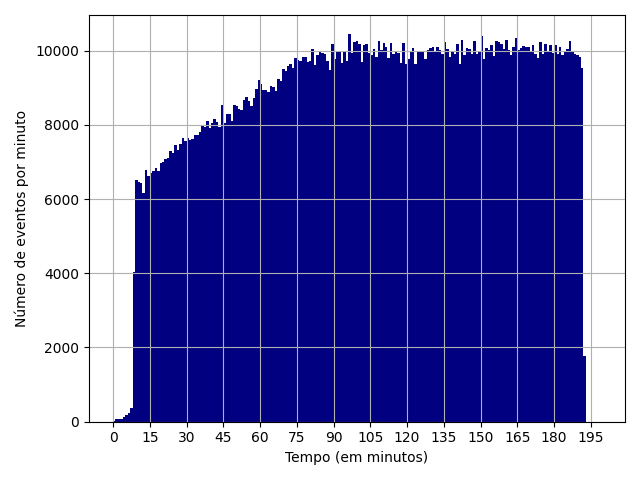
\includegraphics[width=\textwidth]{figuras/graphics/histogram_vazao_5-dez-su.png}
\caption{Vazão de eventos detectados pelo sistema na execução 1 do experimento utilizando o algoritmo de balanceamento por Uso de Estado.}
\label{fig:vazao_5-dez-su}
\end{figure}

%\subsection{Número de instâncias e de eventos de entrada}


\begin{figure}[h]
\centering
\vspace{5cm}
\begin{subfigure}{0.9\textwidth}
\centering
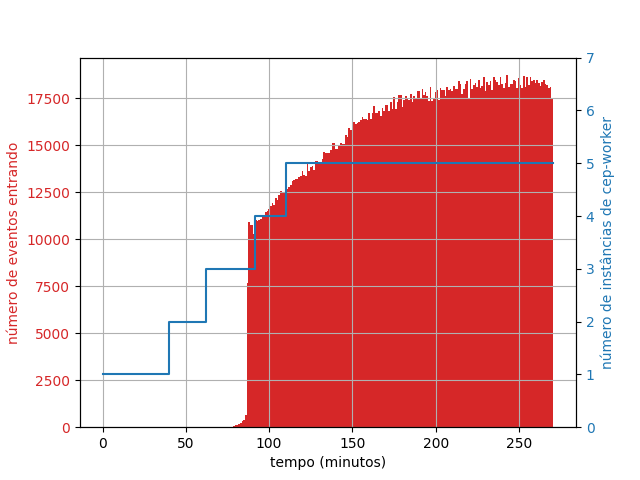
\includegraphics[width=0.8\textwidth]{figuras/graphics/carga_e_workers_total5-dez-su.png}
\caption{Número de eventos entrando no sistema (em vermelho) e número de instâncias de \texttt{CEP Worker} (em azul) em função do tempo na execução 1 do experimento utilizando o algoritmo de balanceamento de carga por Uso de Estado.}
\label{fig:workers_and_load_total}
\end{subfigure}%

\begin{subfigure}{\textwidth}
\centering
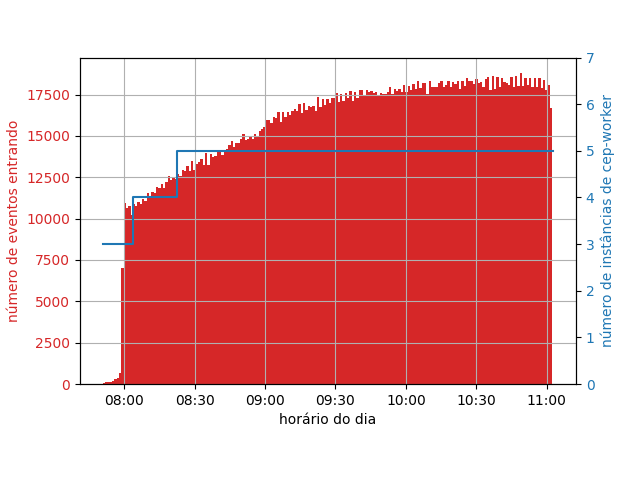
\includegraphics[width=\textwidth]{figuras/graphics/carga_e_workers_horario5-dez-su.png}
\caption{Número de eventos entrando no sistema (em vermelho) e número de instâncias de \texttt{CEP Worker} (em azul) em função do horário do dia na execução 1 do experimento utilizando o algoritmo de balanceamento de carga por Uso de Estado.}
\label{fig:workers_and_load_SPtrans}
\end{subfigure}%
\caption{Número de eventos entrando no sistema e número de instâncias de \texttt{CEP Worker} na execução 1 do experimento utilizando o algoritmo de balanceamento de carga por Uso de Estado.}
\end{figure}

%\subsection{Latência}


\begin{figure}
\centering
\begin{subfigure}{.5\textwidth}
\centering
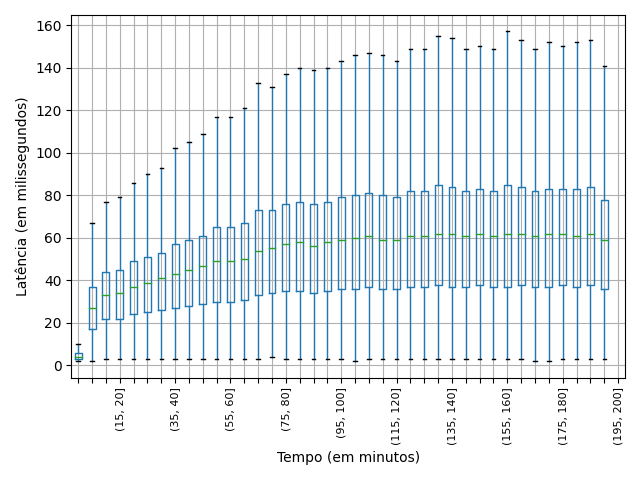
\includegraphics[width=\textwidth]{figuras/graphics/boxplot_5-dez-su_vf.png}
\caption{BoxPlot da latência da categoria de tipos de evento \textbf{vf} por intervalos de cinco minutos ao longo da execução 1 do experimento utilizando o algoritmo de balanceamento de carga por Uso de Estado.}
\label{fig:BoxPlot_vf_SU_1}
\end{subfigure}%
%\end{figure}

%\begin{figure}
\begin{subfigure}{.5\textwidth}
\centering
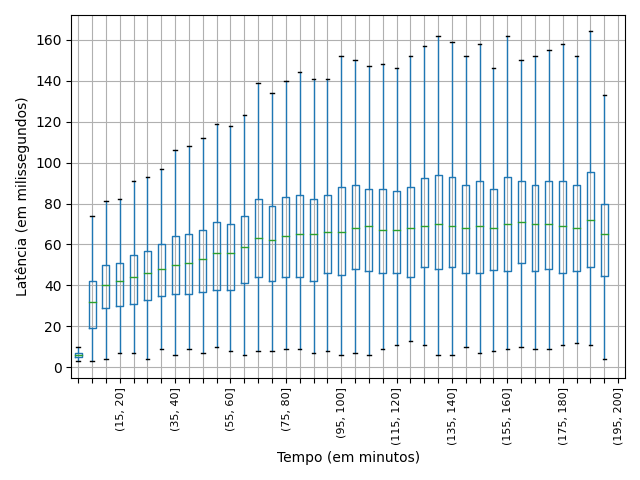
\includegraphics[width=\textwidth]{figuras/graphics/boxplot_5-dez-su_vi.png}
\caption{BoxPlot da latência da categoria de tipos de evento \textbf{vi} por intervalos de cinco minutos ao longo da execução 1 do experimento utilizando o algoritmo de balanceamento de carga por Uso de Estado.}
\label{fig:BoxPlot_vi_SU_1}
\end{subfigure}%
%\end{figure}
\centering
%\begin{figure}
\begin{subfigure}{.5\textwidth}
\centering
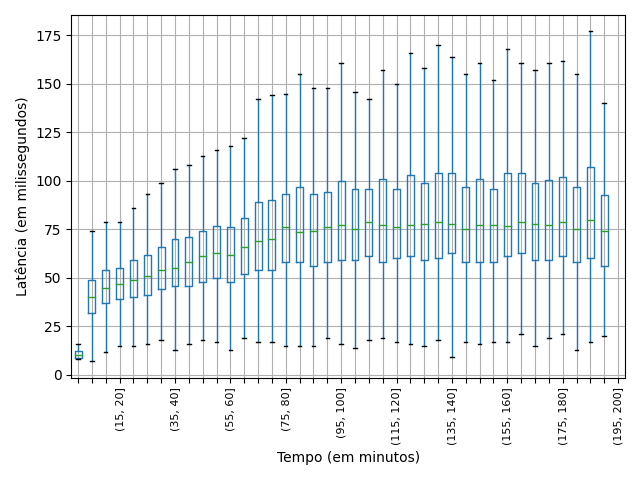
\includegraphics[width=\textwidth]{figuras/graphics/boxplot_5-dez-su_vel.png}
\caption{BoxPlot da latência da categoria de tipos de evento \textbf{vel} por intervalos de cinco minutos ao longo da execução 1 do experimento utilizando o algoritmo de balanceamento de carga por Uso de Estado.}
\label{fig:BoxPlot_vel_SU_1}
\end{subfigure}%
%\end{figure}

%\begin{figure}
\begin{subfigure}{.5\textwidth}
\centering
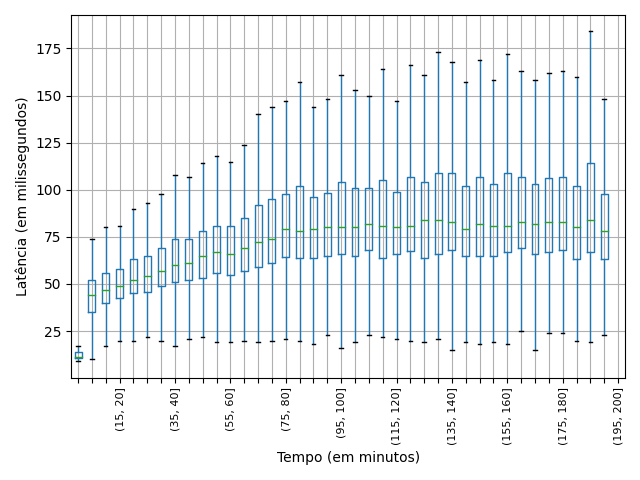
\includegraphics[width=\textwidth]{figuras/graphics/boxplot_5-dez-su_corr.png}
\caption{BoxPlot da latência da categoria de tipos de evento \textbf{corr} por intervalos de cinco minutos ao longo da execução 1 do experimento utilizando o algoritmo de balanceamento de carga por Uso de Estado.}
\label{fig:BoxPlot_corr_SU_1}
\end{subfigure}%
%\end{figure}
%\begin{figure}
\begin{subfigure}{.5\textwidth}
\centering
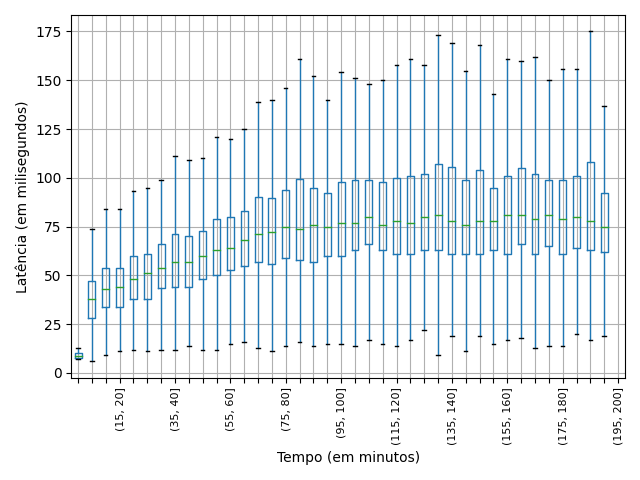
\includegraphics[width=\textwidth]{figuras/graphics/boxplot_5-dez-su_busb.png}
\caption{BoxPlot da latência da categoria de tipos de evento \textbf{BusB} por intervalos de cinco minutos ao longo da execução 1 do experimento utilizando o algoritmo de balanceamento de carga por Uso de Estado.}
\label{fig:BoxPlot_BusB_SU_1}
\end{subfigure}%
\caption{BoxPlot da latência por intervalos de cinco minutos ao longo da execução 1 do experimento utilizando o algoritmo de balanceamento de carga por Uso de Estado.}
\end{figure}






%----------------------------------------
%\newpage
%\section{Experimento 1 - Algoritmo de Similaridade de Entrada}


%\subsection{Vazão}


\begin{figure}[h]
\centering
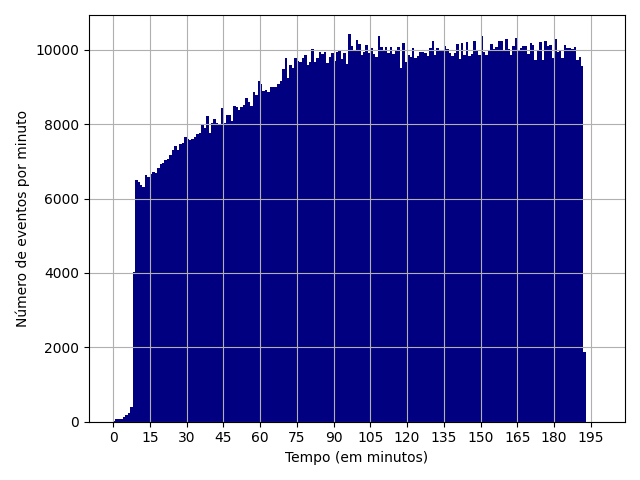
\includegraphics[width=\textwidth]{figuras/graphics/histogram_vazao_6-dez-is.png}
\caption{Vazão de eventos detectados pelo sistema na execução 1 do experimento utilizando o algoritmo de balanceamento por Similaridade de Entrada.}
\label{fig:vazao_6-dez-is}
\end{figure}

%\subsection{Número de instâncias e de eventos de entrada}


\begin{figure}[h]
\centering
\begin{subfigure}{0.9\textwidth}
\centering
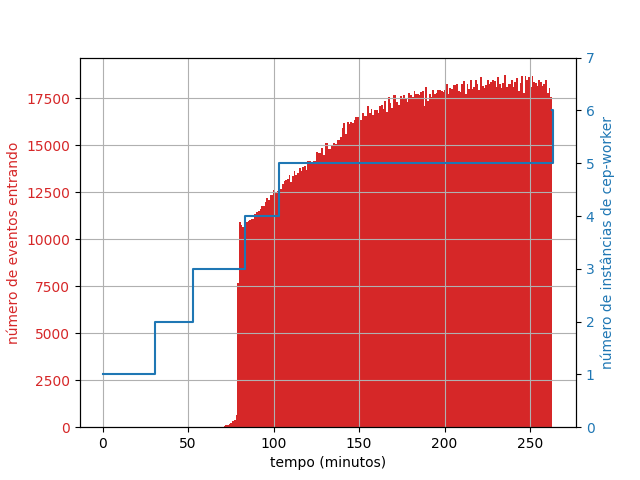
\includegraphics[width=\textwidth]{figuras/graphics/carga_e_workers_total6-dez-is.png}
\caption{Número de eventos entrando no sistema (em vermelho) e número de instâncias de \texttt{CEP Worker} (em azul) em função do tempo na execução 1 do experimento utilizando o algoritmo de balanceamento de carga por Similaridade de Entrada.}
\label{fig:workers_and_load_total-6-dez-is}
\end{subfigure}%

\begin{subfigure}{\textwidth}
\centering
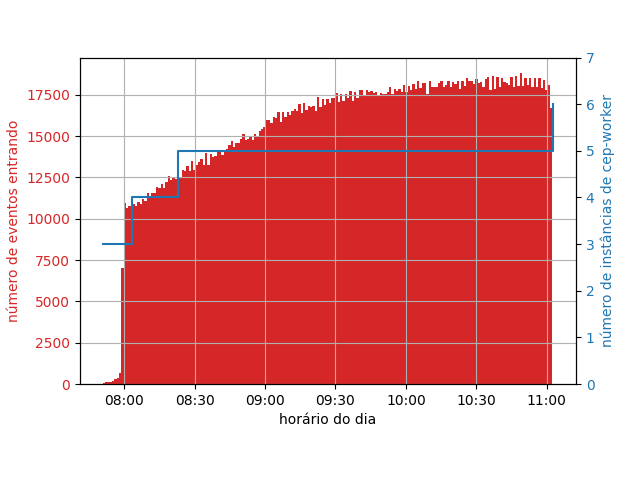
\includegraphics[width=\textwidth]{figuras/graphics/carga_e_workers_horario6-dez-is.png}
\caption{Número de eventos entrando no sistema (em vermelho) e número de instâncias de \texttt{CEP Worker} (em azul) em função do horário do dia na execução 1 do experimento utilizando o algoritmo de balanceamento de carga por Similaridade de Entrada.}
\label{fig:workers_and_load_SPtrans-6-dez-is}
\end{subfigure}%
\caption{Número de eventos entrando no sistema e número de instâncias de \texttt{CEP Worker} na execução 1 do experimento utilizando o algoritmo de balanceamento de carga por Similaridade de Entrada.}
\end{figure}



%\subsection{Latência}


\begin{figure}
\centering
\begin{subfigure}{.5\textwidth}
\centering
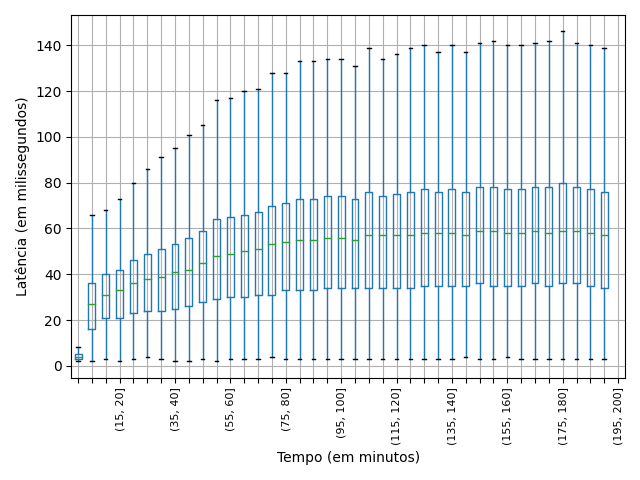
\includegraphics[width=\textwidth]{figuras/graphics/boxplot_6-dez-is_vf.png}
\caption{BoxPlot da latência da categoria de tipos de evento \textbf{vf} por intervalos de cinco minutos ao longo da execução 1 do experimento utilizando o algoritmo de balanceamento de carga por Similaridade de Entrada.}
\label{fig:BoxPlot_vf_IS_1}
\end{subfigure}%
%\end{figure}

%\begin{figure}
\begin{subfigure}{.5\textwidth}
\centering
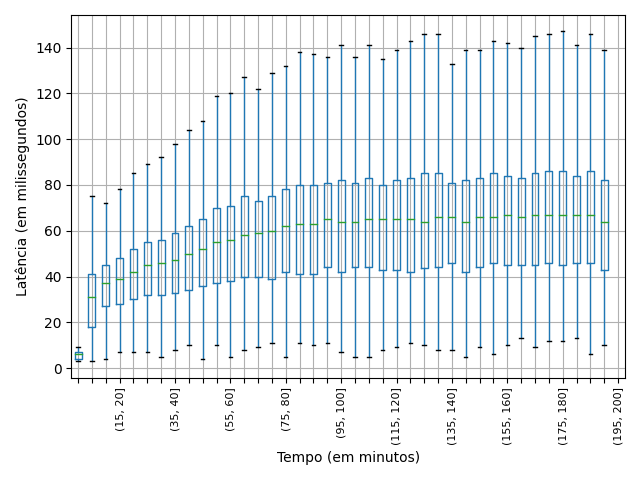
\includegraphics[width=\textwidth]{figuras/graphics/boxplot_6-dez-is_vi.png}
\caption{BoxPlot da latência da categoria de tipos de evento \textbf{vi} por intervalos de cinco minutos ao longo da execução 1 do experimento utilizando o algoritmo de balanceamento de carga por Similaridade de Entrada.}
\label{fig:BoxPlot_vi_IS_1}
\end{subfigure}%
%\end{figure}
\centering
%\begin{figure}
\begin{subfigure}{.5\textwidth}
\centering
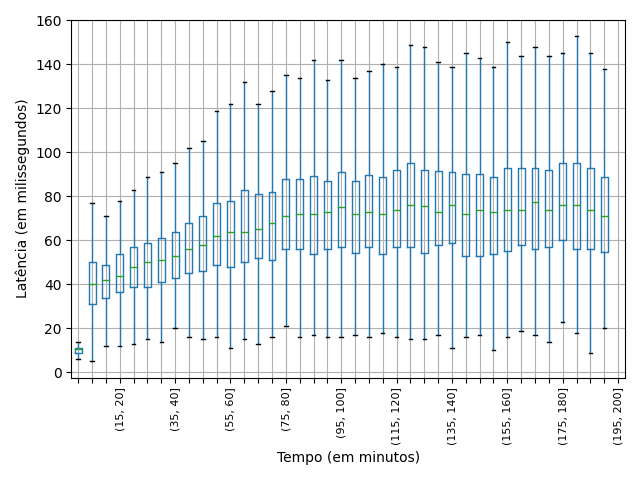
\includegraphics[width=\textwidth]{figuras/graphics/boxplot_6-dez-is_vel.png}
\caption{BoxPlot da latência da categoria de tipos de evento \textbf{vel} por intervalos de cinco minutos ao longo da execução 1 do experimento utilizando o algoritmo de balanceamento de carga por Similaridade de Entrada.}
\label{fig:BoxPlot_vel_IS_1}
\end{subfigure}%
%\end{figure}

%\begin{figure}
\begin{subfigure}{.5\textwidth}
\centering
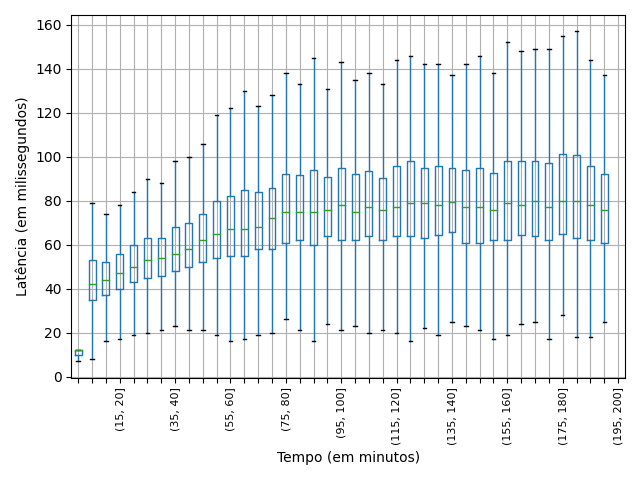
\includegraphics[width=\textwidth]{figuras/graphics/boxplot_6-dez-is_corr.png}
\caption{BoxPlot da latência da categoria de tipos de evento \textbf{corr} por intervalos de cinco minutos ao longo da execução 1 do experimento utilizando o algoritmo de balanceamento de carga por Similaridade de Entrada.}
\label{fig:BoxPlot_corr_IS_1}
\end{subfigure}%
%\end{figure}
%\begin{figure}
\begin{subfigure}{.5\textwidth}
\centering
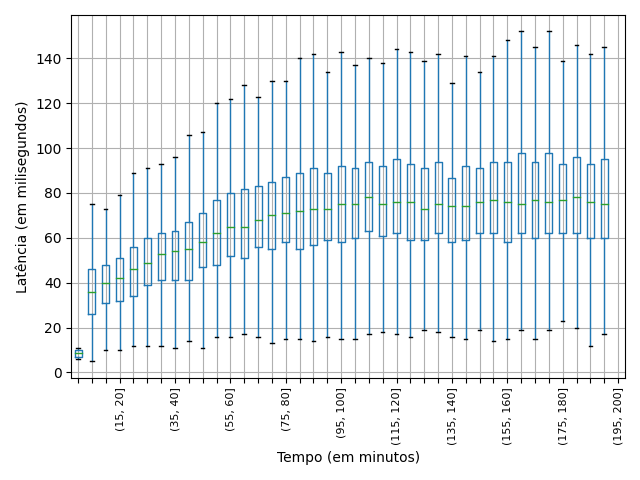
\includegraphics[width=\textwidth]{figuras/graphics/boxplot_6-dez-is_busb.png}
\caption{BoxPlot da latência da categoria de tipos de evento \textbf{BusB} por intervalos de cinco minutos ao longo da execução 1 do experimento utilizando o algoritmo de balanceamento de carga por Similaridade de Entrada.}
\label{fig:BoxPlot_BusB_IS_1}
\end{subfigure}%
\caption{BoxPlot da latência por intervalos de cinco minutos ao longo da execução 1 do experimento utilizando o algoritmo de balanceamento de carga por Similaridade de Entrada.}
\end{figure}




%\newpage

%------------------------------------------------

%\section{Experimento 2 - Algoritmo de Uso de Estado}

%\subsection{Vazão}


\begin{figure}[h]
\centering
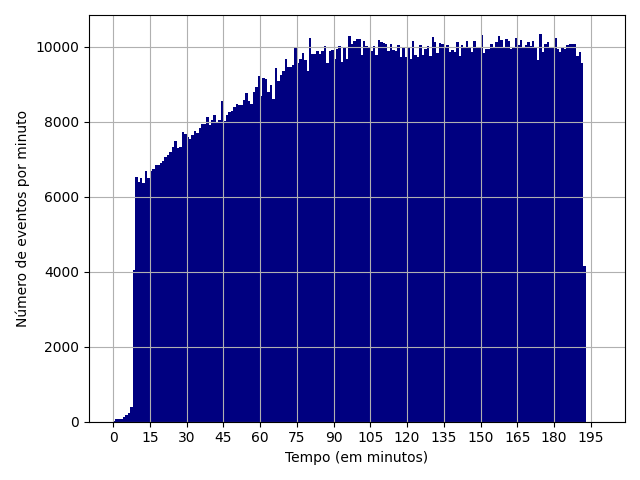
\includegraphics[width=\textwidth]{figuras/graphics/histogram_vazao_7-dez-su.png}
\caption{Vazão de eventos detectados pelo sistema na execução 2 do experimento utilizando o algoritmo de balanceamento por Uso de Estado.}
\label{fig:vazao_7-dez-su}
\end{figure}


%\subsection{Número de instâncias e de eventos de entrada}


\begin{figure}[h]
\centering
\begin{subfigure}{0.9\textwidth}
\centering
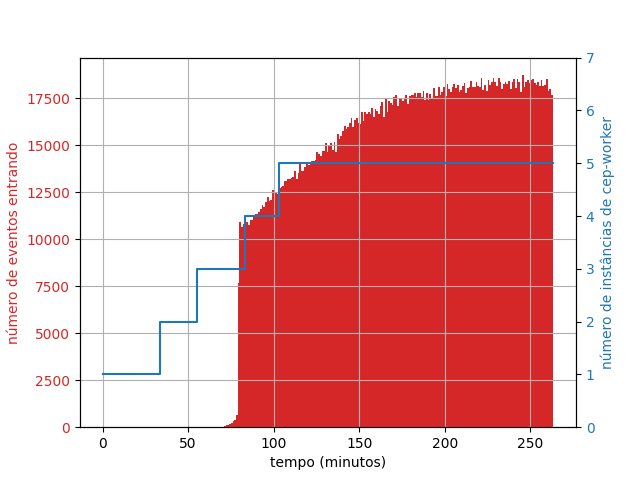
\includegraphics[width=\textwidth]{figuras/graphics/carga_e_workers_total7-dez-su.png}
\caption{Número de eventos entrando no sistema (em vermelho) e número de instâncias de \texttt{CEP Worker} (em azul) em função do tempo na execução 2 do experimento utilizando o algoritmo de balanceamento de carga por Uso de Estado.}
\label{fig:workers_and_load_total_7-dez-su}
\end{subfigure}%

\begin{subfigure}{\textwidth}
\centering
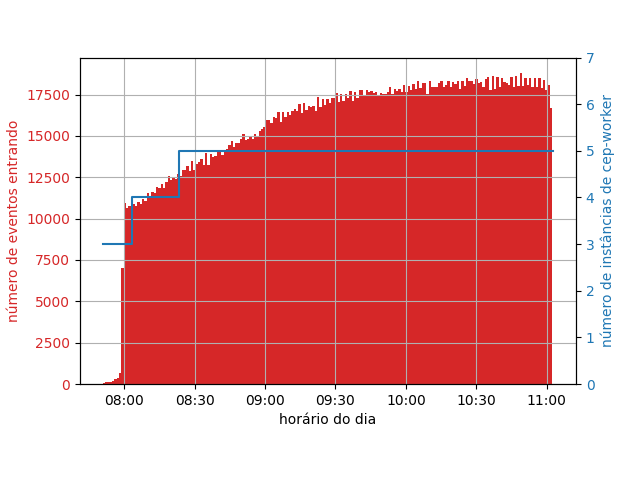
\includegraphics[width=\textwidth]{figuras/graphics/carga_e_workers_horario7-dez-su.png}
\caption{Número de eventos entrando no sistema (em vermelho) e número de instâncias de \texttt{CEP Worker} (em azul) em função do horário do dia na execução 2 do experimento utilizando o algoritmo de balanceamento de carga por Uso de Estado.}
\label{fig:workers_and_load_SPtrans_7-dez-su}
\end{subfigure}%
\caption{Número de eventos entrando no sistema e número de instâncias de \texttt{CEP Worker} na execução 2 do experimento utilizando o algoritmo de balanceamento de carga por Uso de Estado.}
\end{figure}


%\subsection{Latência}


\begin{figure}
\centering
\begin{subfigure}{.5\textwidth}
\centering
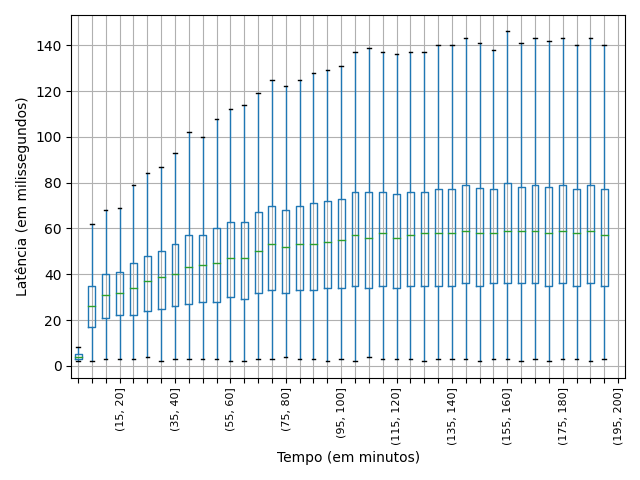
\includegraphics[width=\textwidth]{figuras/graphics/boxplot_7-dez-su_vf.png}
\caption{BoxPlot da latência da categoria de tipos de evento \textbf{vf} por intervalos de cinco minutos ao longo da execução 2 do experimento utilizando o algoritmo de balanceamento de carga por Uso de Estado.}
\label{fig:BoxPlot_vf_SU_7-dez-su}
\end{subfigure}%
%\end{figure}

%\begin{figure}
\begin{subfigure}{.5\textwidth}
\centering
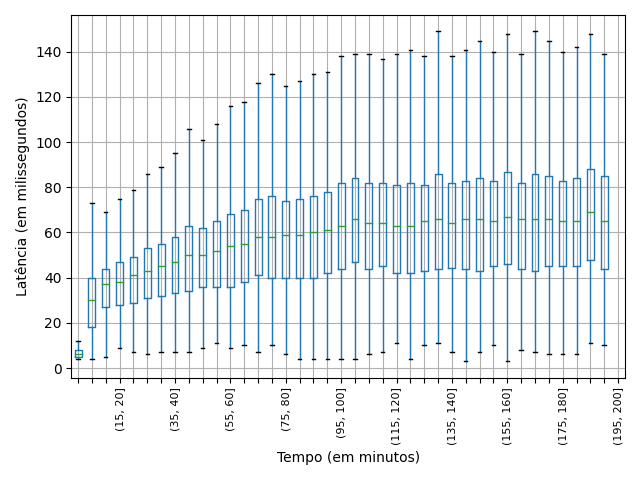
\includegraphics[width=\textwidth]{figuras/graphics/boxplot_7-dez-su_vi.png}
\caption{BoxPlot da latência da categoria de tipos de evento \textbf{vi} por intervalos de cinco minutos ao longo da execução 2 do experimento utilizando o algoritmo de balanceamento de carga por Uso de Estado.}
\label{fig:BoxPlot_vi_SU_7-dez-su}
\end{subfigure}%
%\end{figure}
\centering
%\begin{figure}
\begin{subfigure}{.5\textwidth}
\centering
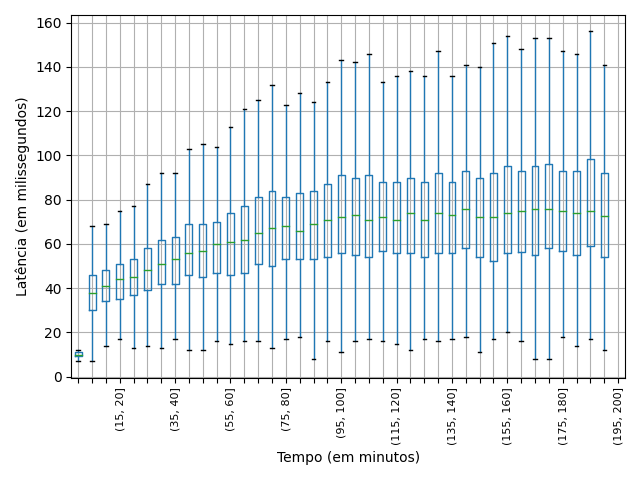
\includegraphics[width=\textwidth]{figuras/graphics/boxplot_7-dez-su_vel.png}
\caption{BoxPlot da latência da categoria de tipos de evento \textbf{vel} por intervalos de cinco minutos ao longo da execução 2 do experimento utilizando o algoritmo de balanceamento de carga por Uso de Estado.}
\label{fig:BoxPlot_vel_SU_7-dez-su}
\end{subfigure}%
%\end{figure}

%\begin{figure}
\begin{subfigure}{.5\textwidth}
\centering
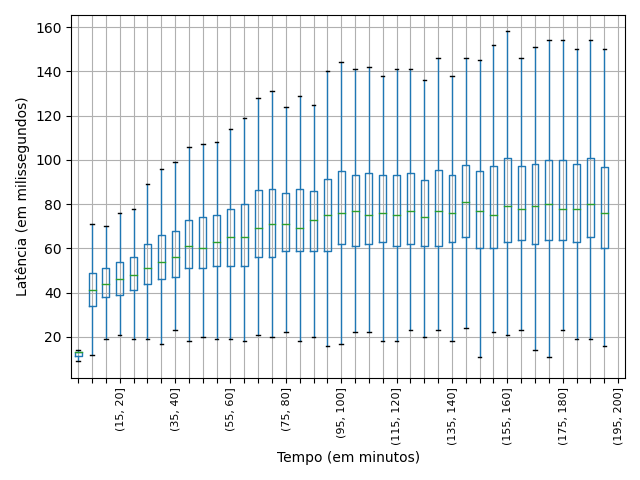
\includegraphics[width=\textwidth]{figuras/graphics/boxplot_7-dez-su_corr.png}
\caption{BoxPlot da latência da categoria de tipos de evento \textbf{corr} por intervalos de cinco minutos ao longo da execução 2 do experimento utilizando o algoritmo de balanceamento de carga por Uso de Estado.}
\label{fig:BoxPlot_corr_SU_7-dez-su}
\end{subfigure}%
%\end{figure}
%\begin{figure}
\begin{subfigure}{.5\textwidth}
\centering
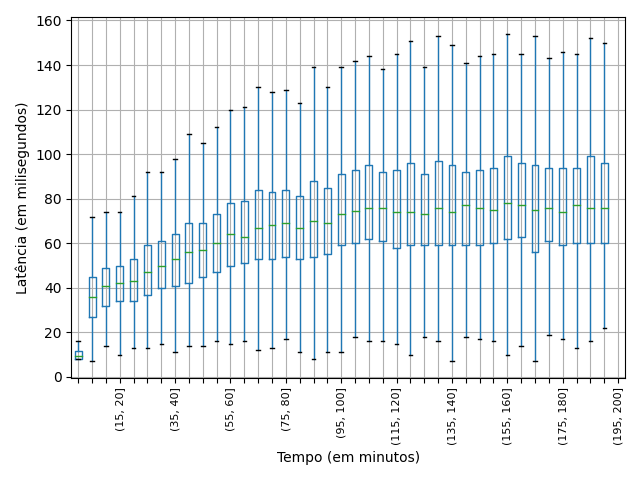
\includegraphics[width=\textwidth]{figuras/graphics/boxplot_7-dez-su_busb.png}
\caption{BoxPlot da latência da categoria de tipos de evento \textbf{BusB} por intervalos de cinco minutos ao longo da execução 2 do experimento utilizando o algoritmo de balanceamento de carga por Uso de Estado.}
\label{fig:BoxPlot_BusB_SU_7-dez-su}
\end{subfigure}%
\caption{BoxPlot da latência por intervalos de cinco minutos ao longo da execução 2 do experimento utilizando o algoritmo de balanceamento de carga por Uso de Estado.}
\end{figure}






%----------------------------------------
%\newpage
%\section{Experimento 2 - Algoritmo de Similaridade de Entrada}

%\subsection{Vazão}


\begin{figure}[h]
\centering
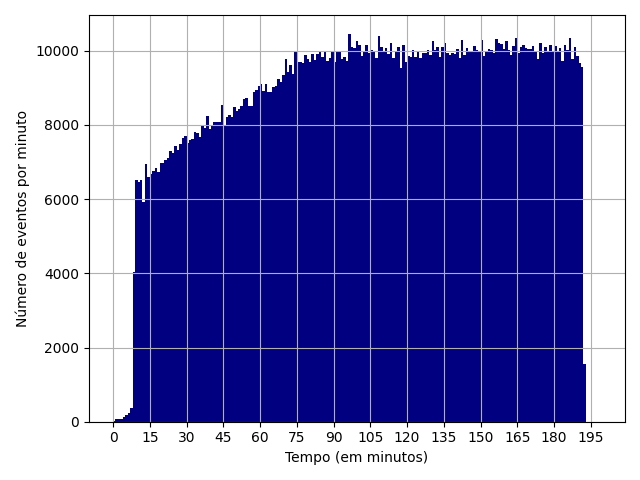
\includegraphics[width=\textwidth]{figuras/graphics/histogram_vazao_7-dez-is.png}
\caption{Vazão de eventos detectados pelo sistema na execução 2 do experimento utilizando o algoritmo de balanceamento por Similaridade de Entrada.}
\label{fig:vazao_7-dez-is}
\end{figure}

%\subsection{Número de instâncias e de eventos de entrada}


\begin{figure}[h]
\centering
\begin{subfigure}{0.9\textwidth}
\centering
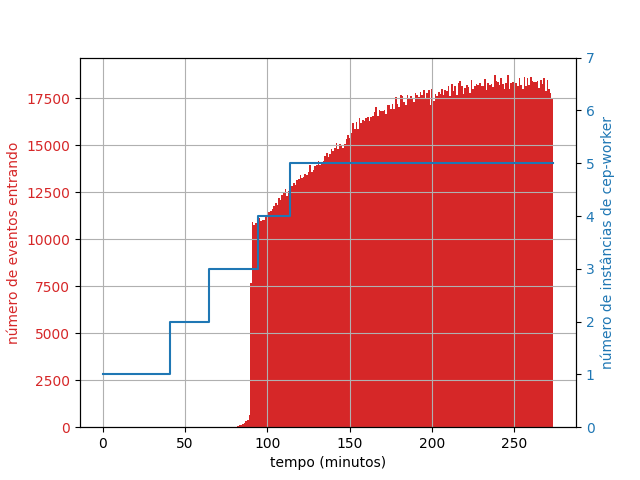
\includegraphics[width=\textwidth]{figuras/graphics/carga_e_workers_total7-dez-is.png}
\caption{Número de eventos entrando no sistema (em vermelho) e número de instâncias de \texttt{CEP Worker} (em azul) em função do tempo na execução 2 do experimento utilizando o algoritmo de balanceamento de carga por Similaridade de Entrada.}
\label{fig:workers_and_load_total-7-dez-is}
\end{subfigure}%

\begin{subfigure}{\textwidth}
\centering
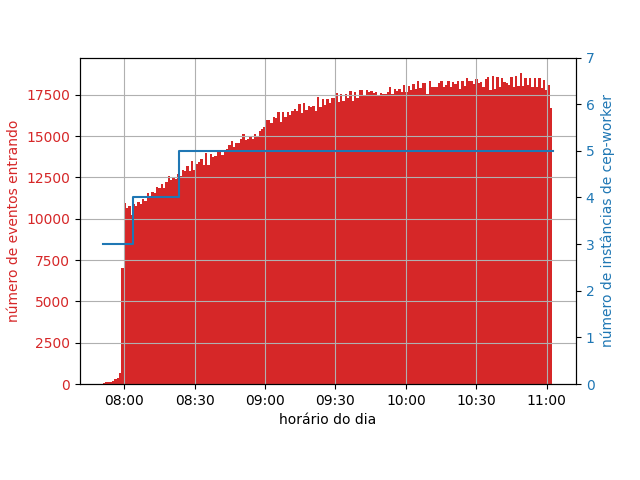
\includegraphics[width=\textwidth]{figuras/graphics/carga_e_workers_horario7-dez-is.png}
\caption{Número de eventos entrando no sistema (em vermelho) e número de instâncias de \texttt{CEP Worker} (em azul) em função do horário do dia na execução 2 do experimento utilizando o algoritmo de balanceamento de carga por Similaridade de Entrada.}
\label{fig:workers_and_load_SPtrans-7-dez-is}
\end{subfigure}%
\caption{Número de eventos entrando no sistema e número de instâncias de \texttt{CEP Worker} na execução 2 do experimento utilizando o algoritmo de balanceamento de carga por Similaridade de Entrada.}
\end{figure}






%\subsection{Latência}


\begin{figure}
\centering
\begin{subfigure}{.5\textwidth}
\centering
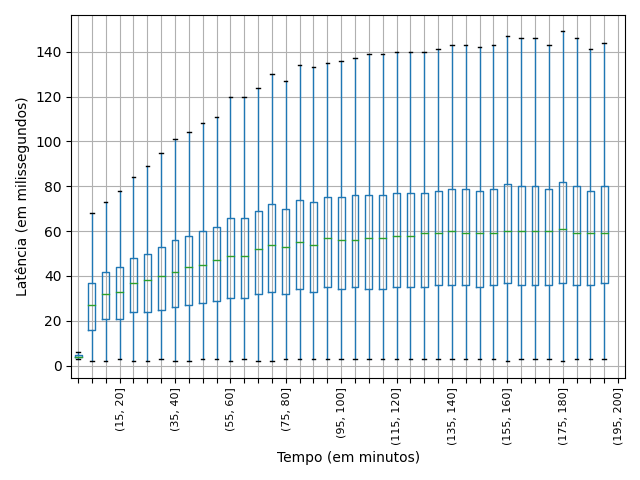
\includegraphics[width=\textwidth]{figuras/graphics/boxplot_7-dez-is_vf.png}
\caption{BoxPlot da latência da categoria de tipos de evento \textbf{vf} por intervalos de cinco minutos ao longo da execução  2 do experimento utilizando o algoritmo de balanceamento de carga por Similaridade de Entrada.}
\label{fig:BoxPlot_vf_7-dez-is}
\end{subfigure}%
%\end{figure}

%\begin{figure}
\begin{subfigure}{.5\textwidth}
\centering
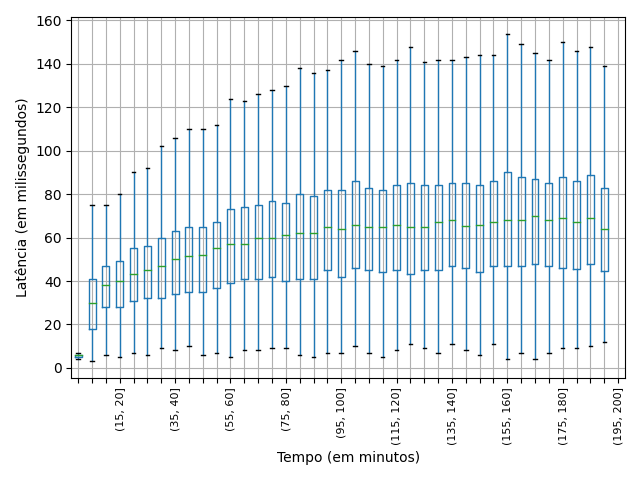
\includegraphics[width=\textwidth]{figuras/graphics/boxplot_7-dez-is_vi.png}
\caption{BoxPlot da latência da categoria de tipos de evento \textbf{vi} por intervalos de cinco minutos ao longo da execução 2 do experimento utilizando o algoritmo de balanceamento de carga por Similaridade de Entrada.}
\label{fig:BoxPlot_vi_IS_7-dez-is}
\end{subfigure}%
%\end{figure}
\centering
%\begin{figure}
\begin{subfigure}{.5\textwidth}
\centering
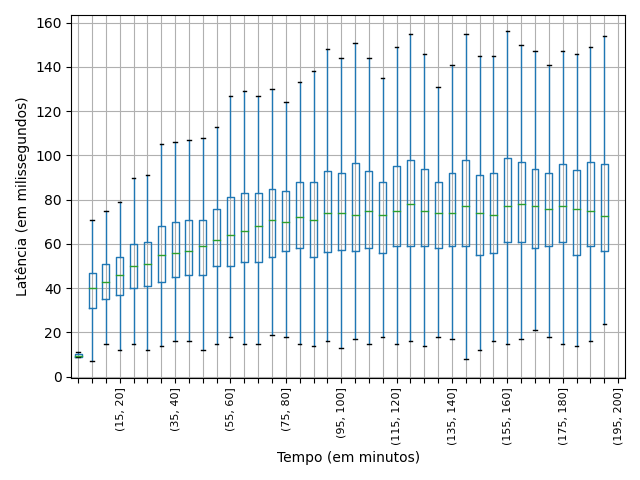
\includegraphics[width=\textwidth]{figuras/graphics/boxplot_7-dez-is_vel.png}
\caption{BoxPlot da latência da categoria de tipos de evento \textbf{vel} por intervalos de cinco minutos ao longo da execução 2 do experimento utilizando o algoritmo de balanceamento de carga por Similaridade de Entrada.}
\label{fig:BoxPlot_vel_IS_7-dez-is}
\end{subfigure}%
%\end{figure}

%\begin{figure}
\begin{subfigure}{.5\textwidth}
\centering
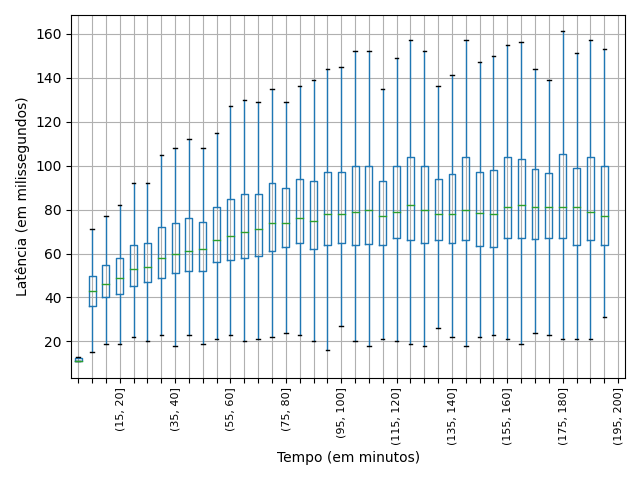
\includegraphics[width=\textwidth]{figuras/graphics/boxplot_7-dez-is_corr.png}
\caption{BoxPlot da latência da categoria de tipos de evento \textbf{corr} por intervalos de cinco minutos ao longo da execução 2 do experimento utilizando o algoritmo de balanceamento de carga por Similaridade de Entrada.}
\label{fig:BoxPlot_corr_IS_7-dez-is}
\end{subfigure}%
%\end{figure}
%\begin{figure}
\begin{subfigure}{.5\textwidth}
\centering
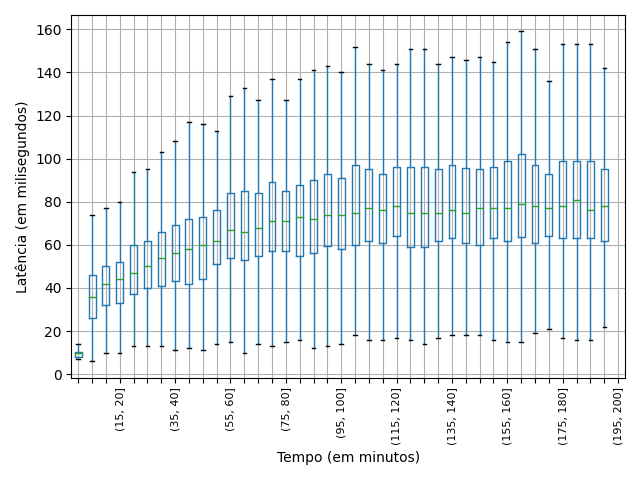
\includegraphics[width=\textwidth]{figuras/graphics/boxplot_7-dez-is_busb.png}
\caption{BoxPlot da latência da categoria de tipos de evento \textbf{BusB} por intervalos de cinco minutos ao longo da execução 2 do experimento utilizando o algoritmo de balanceamento de carga por Similaridade de Entrada.}
\label{fig:BoxPlot_BusB_IS_7-dez-is}
\end{subfigure}%
\caption{BoxPlot da latência por intervalos de cinco minutos ao longo da execução 2 do experimento utilizando o algoritmo de balanceamento de carga por Similaridade de Entrada.}
\end{figure}


%\newpage

%----------------------------------------------------------------


%\section{Experimento 3 - Algoritmo de Uso de Estado}

%\subsection{Vazão}


\begin{figure}[h]
\centering
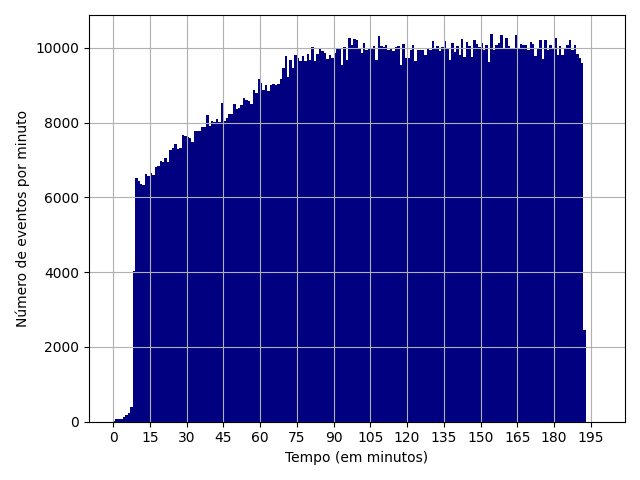
\includegraphics[width=\textwidth]{figuras/graphics/histogram_vazao_8-dez-su.png}
\caption{Vazão de eventos detectados pelo sistema na execução 3 do experimento utilizando o algoritmo de balanceamento por Uso de Estado.}
\label{fig:vazao_8-dez-su}
\end{figure}

%\subsection{Número de instâncias e de eventos de entrada}


\begin{figure}[h]
\centering
\begin{subfigure}{0.9\textwidth}
\centering
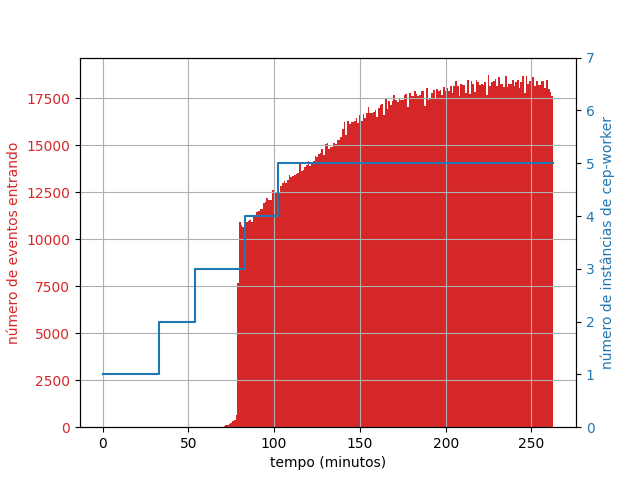
\includegraphics[width=\textwidth]{figuras/graphics/carga_e_workers_total8-dez-su.png}
\caption{Número de eventos entrando no sistema (em vermelho) e número de instâncias de \texttt{CEP Worker} (em azul) em função do tempo na execução 3 do experimento utilizando o algoritmo de balanceamento de carga por Uso de Estado.}
\label{fig:workers_and_load_total_8-dez-su}
\end{subfigure}%

\begin{subfigure}{\textwidth}
\centering
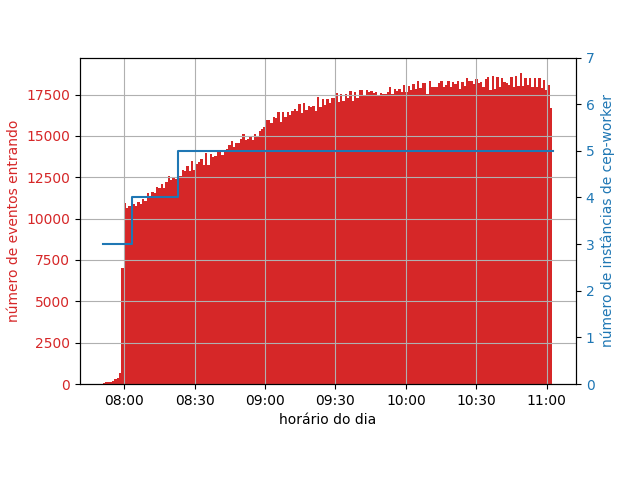
\includegraphics[width=\textwidth]{figuras/graphics/carga_e_workers_horario8-dez-su.png}
\caption{Número de eventos entrando no sistema (em vermelho) e número de instâncias de \texttt{CEP Worker} (em azul) em função do horário do dia na execução 3 do experimento utilizando o algoritmo de balanceamento de carga por Uso de Estado.}
\label{fig:workers_and_load_SPtrans_8-dez-su}
\end{subfigure}%
\caption{Número de eventos entrando no sistema e número de instâncias de \texttt{CEP Worker} na execução 3 do experimento utilizando o algoritmo de balanceamento de carga por Uso de Estado.}
\end{figure}

%\subsection{Latência}


\begin{figure}
\centering
\begin{subfigure}{.5\textwidth}
\centering
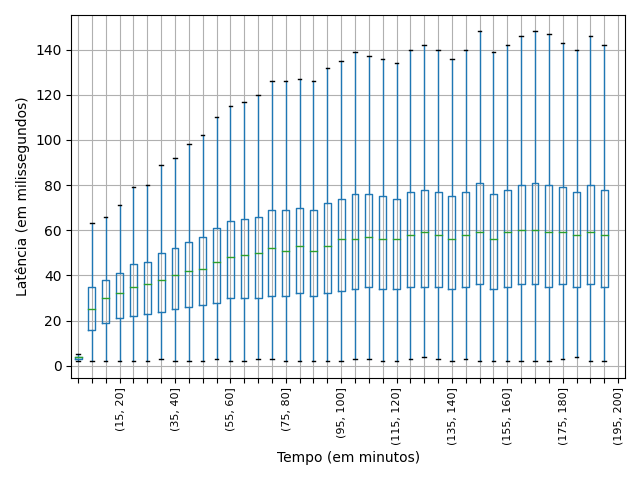
\includegraphics[width=\textwidth]{figuras/graphics/boxplot_8-dez-su_vf.png}
\caption{BoxPlot da latência da categoria de tipos de evento \textbf{vf} por intervalos de cinco minutos ao longo da execução 3 do experimento utilizando o algoritmo de balanceamento de carga por Uso de Estado.}
\label{fig:BoxPlot_vf_SU_8-dez-su}
\end{subfigure}%
%\end{figure}

%\begin{figure}
\begin{subfigure}{.5\textwidth}
\centering
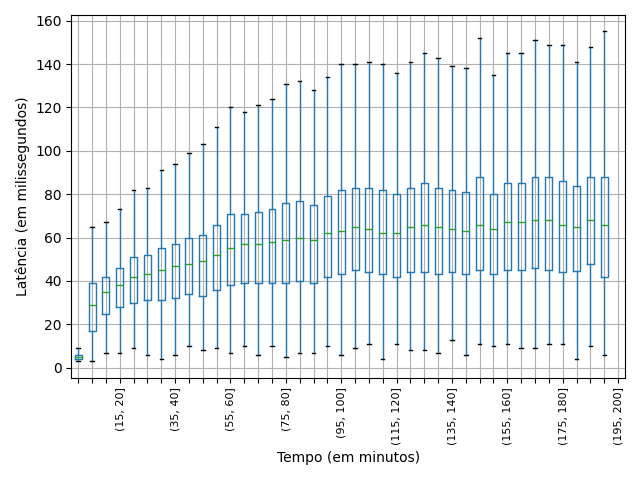
\includegraphics[width=\textwidth]{figuras/graphics/boxplot_8-dez-su_vi.png}
\caption{BoxPlot da latência da categoria de tipos de evento \textbf{vi} por intervalos de cinco minutos ao longo da execução 3 do experimento utilizando o algoritmo de balanceamento de carga por Uso de Estado.}
\label{fig:BoxPlot_vi_SU_8-dez-su}
\end{subfigure}%
%\end{figure}
\centering
%\begin{figure}
\begin{subfigure}{.5\textwidth}
\centering
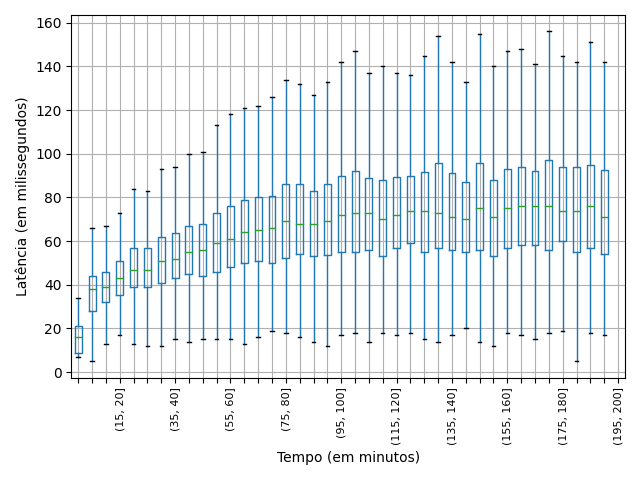
\includegraphics[width=\textwidth]{figuras/graphics/boxplot_8-dez-su_vel.png}
\caption{BoxPlot da latência da categoria de tipos de evento \textbf{vel} por intervalos de cinco minutos ao longo da execução 3 do experimento utilizando o algoritmo de balanceamento de carga por Uso de Estado.}
\label{fig:BoxPlot_vel_SU_8-dez-su}
\end{subfigure}%
%\end{figure}

%\begin{figure}
\begin{subfigure}{.5\textwidth}
\centering
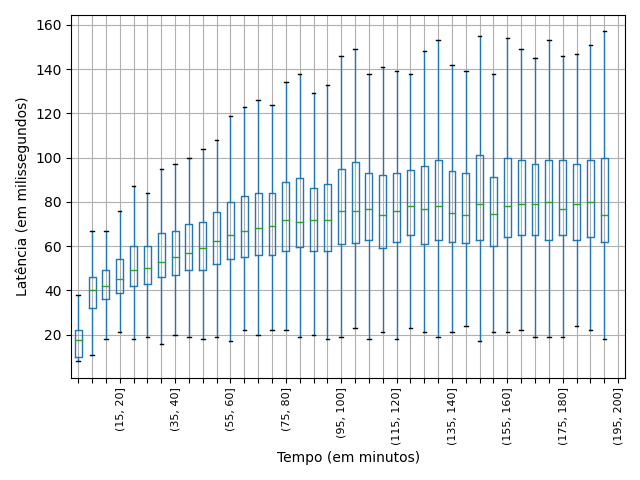
\includegraphics[width=\textwidth]{figuras/graphics/boxplot_8-dez-su_corr.png}
\caption{BoxPlot da latência da categoria de tipos de evento \textbf{corr} por intervalos de cinco minutos ao longo da execução 3 do experimento utilizando o algoritmo de balanceamento de carga por Uso de Estado.}
\label{fig:BoxPlot_corr_SU_8-dez-su}
\end{subfigure}%
%\end{figure}
%\begin{figure}
\begin{subfigure}{.5\textwidth}
\centering
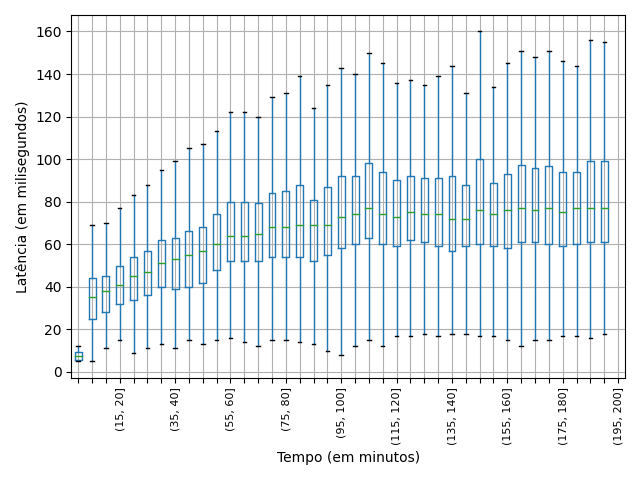
\includegraphics[width=\textwidth]{figuras/graphics/boxplot_8-dez-su_busb.png}
\caption{BoxPlot da latência da categoria de tipos de evento \textbf{BusB} por intervalos de cinco minutos ao longo da execução 3 do experimento utilizando o algoritmo de balanceamento de carga por Uso de Estado.}
\label{fig:BoxPlot_BusB_SU_8-dez-su}
\end{subfigure}%
\caption{BoxPlot da latência por intervalos de cinco minutos ao longo da execução 3 do experimento utilizando o algoritmo de balanceamento de carga por Uso de Estado.}
\end{figure}






%----------------------------------------
%\newpage
%\section{Experimento 3 - Algoritmo de Similaridade de Entrada}

%\subsection{Vazão}


\begin{figure}[h]
\centering
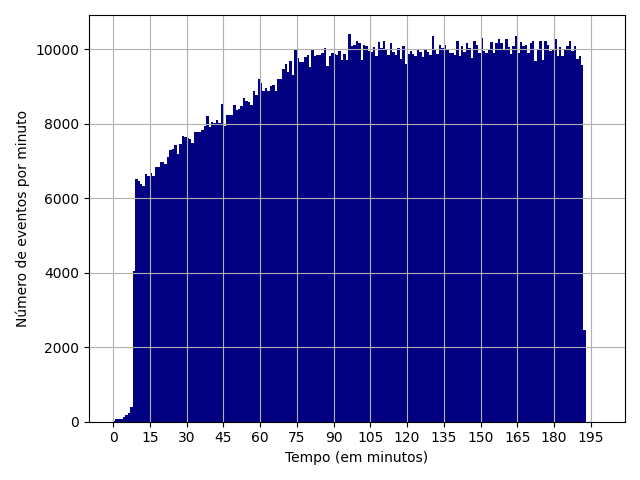
\includegraphics[width=\textwidth]{figuras/graphics/histogram_vazao_8-dez-is.png}
\caption{Vazão de eventos detectados pelo sistema na execução 3 do experimento utilizando o algoritmo de balanceamento por Similaridade de Entrada.}
\label{fig:vazao_8-dez-is}
\end{figure}

%\subsection{Número de instâncias e de eventos de entrada}


\begin{figure}[h]
\centering
\begin{subfigure}{0.9\textwidth}
\centering
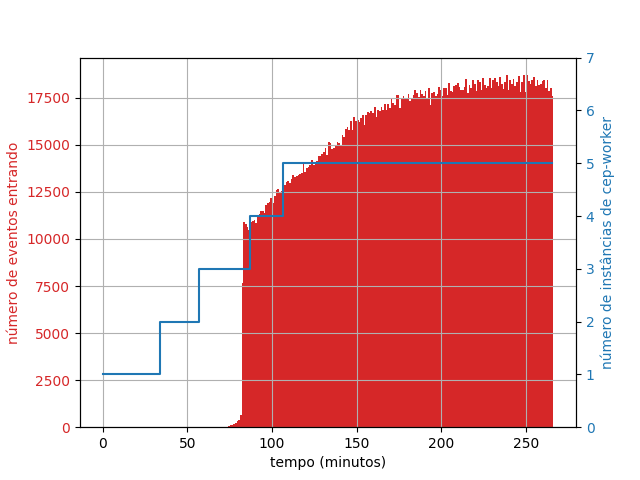
\includegraphics[width=\textwidth]{figuras/graphics/carga_e_workers_total8-dez-is.png}
\caption{Número de eventos entrando no sistema (em vermelho) e número de instâncias de \texttt{CEP Worker} (em azul) em função do tempo na execução 3 do experimento utilizando o algoritmo de balanceamento de carga por Similaridade de Entrada.}
\label{fig:workers_and_load_total-8-dez-is}
\end{subfigure}%

\begin{subfigure}{\textwidth}
\centering
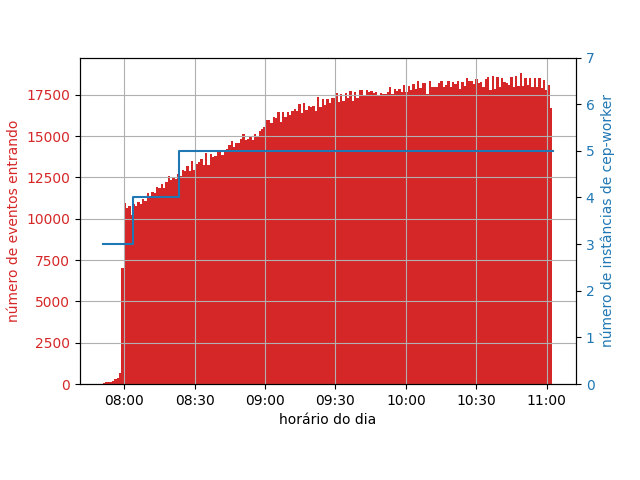
\includegraphics[width=\textwidth]{figuras/graphics/carga_e_workers_horario8-dez-is.png}
\caption{Número de eventos entrando no sistema (em vermelho) e número de instâncias de \texttt{CEP Worker} (em azul) em função do horário do dia na execução 3 do experimento utilizando o algoritmo de balanceamento de carga por Similaridade de Entrada.}
\label{fig:workers_and_load_SPtrans-8-dez-is}
\end{subfigure}%
\caption{Número de eventos entrando no sistema e número de instâncias de \texttt{CEP Worker} na execução 3 do experimento utilizando o algoritmo de balanceamento de carga por Similaridade de Entrada.}
\end{figure}




%\subsection{Latência}


\begin{figure}
\centering
\begin{subfigure}{.5\textwidth}
\centering
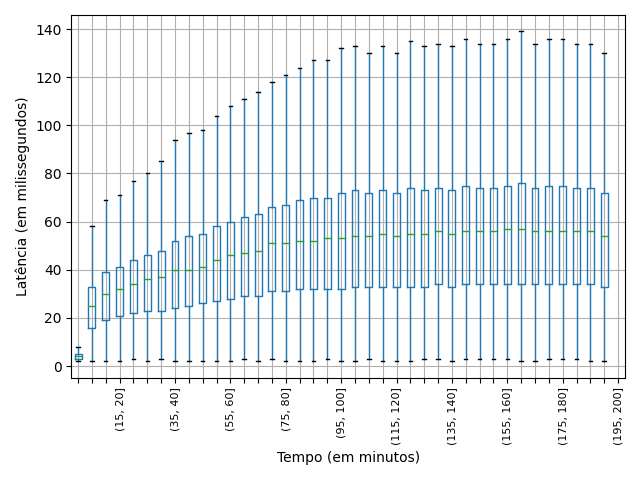
\includegraphics[width=\textwidth]{figuras/graphics/boxplot_8-dez-is_vf.png}
\caption{BoxPlot da latência da categoria de tipos de evento \textbf{vf} por intervalos de cinco minutos ao longo da execução 3 do experimento utilizando o algoritmo de balanceamento por Similaridade de Entrada.}
\label{fig:BoxPlot_vf_8-dez-is}
\end{subfigure}%
%\end{figure}

%\begin{figure}
\begin{subfigure}{.5\textwidth}
\centering
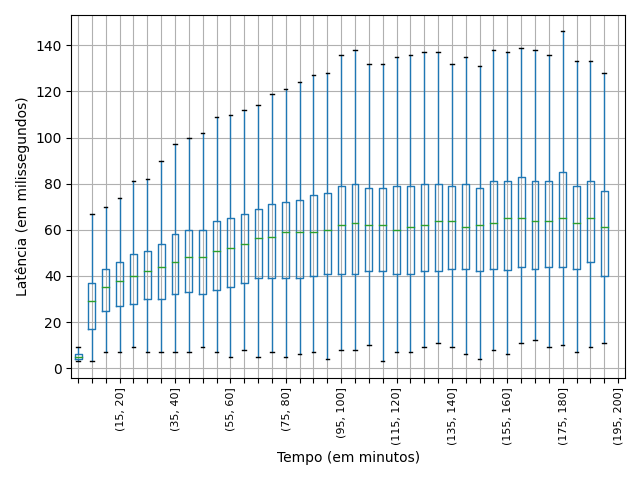
\includegraphics[width=\textwidth]{figuras/graphics/boxplot_8-dez-is_vi.png}
\caption{BoxPlot da latência da categoria de tipos de evento \textbf{vi} por intervalos de cinco minutos ao longo da execução 3 do experimento utilizando o algoritmo de balanceamento por Similaridade de Entrada.}
\label{fig:BoxPlot_vi_IS_8-dez-is}
\end{subfigure}%
%\end{figure}
\centering
%\begin{figure}
\begin{subfigure}{.5\textwidth}
\centering
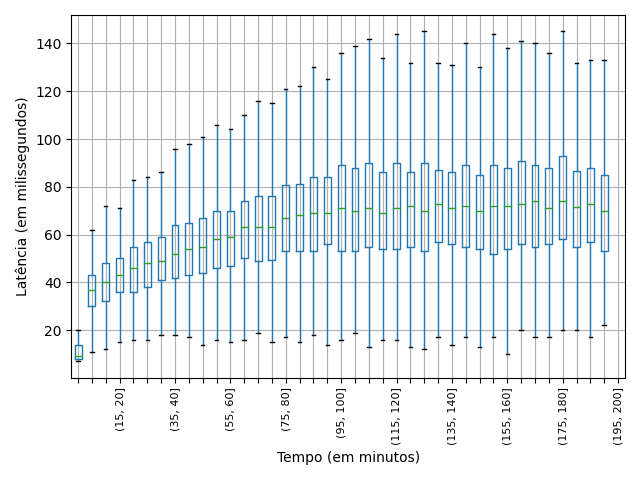
\includegraphics[width=\textwidth]{figuras/graphics/boxplot_8-dez-is_vel.png}
\caption{BoxPlot da latência da categoria de tipos de evento \textbf{vel} por intervalos de cinco minutos ao longo da execução 3 do experimento utilizando o algoritmo de balanceamento por Similaridade de Entrada.}
\label{fig:BoxPlot_vel_IS_8-dez-is}
\end{subfigure}%
%\end{figure}

%\begin{figure}
\begin{subfigure}{.5\textwidth}
\centering
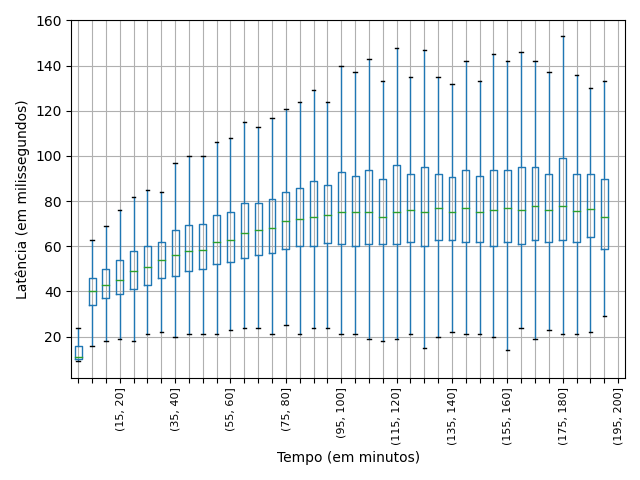
\includegraphics[width=\textwidth]{figuras/graphics/boxplot_8-dez-is_corr.png}
\caption{BoxPlot da latência da categoria de tipos de evento \textbf{corr} por intervalos de cinco minutos ao longo da execução 3 do experimento utilizando o algoritmo de balanceamento por Similaridade de Entrada.}
\label{fig:BoxPlot_corr_IS_8-dez-is}
\end{subfigure}%
%\end{figure}
%\begin{figure}
\begin{subfigure}{.5\textwidth}
\centering
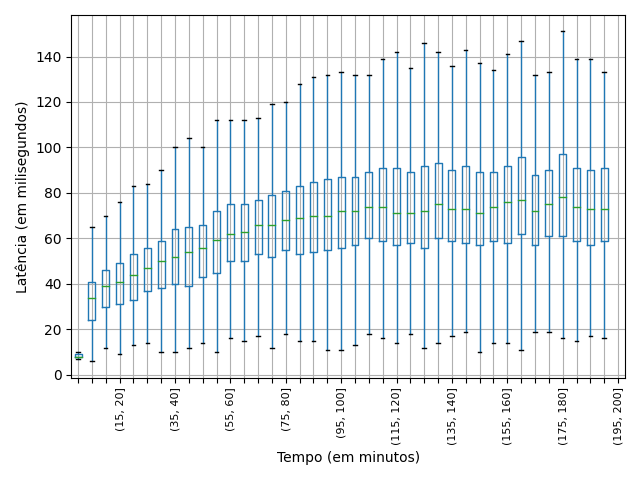
\includegraphics[width=\textwidth]{figuras/graphics/boxplot_8-dez-is_busb.png}
\caption{BoxPlot da latência da categoria de tipos de evento \textbf{BusB} por intervalos de cinco minutos ao longo da execução 3 do experimento utilizando o algoritmo de balanceamento por Similaridade de Entrada.}
\label{fig:BoxPlot_BusB_IS_8-dez-is}
\end{subfigure}%
\caption{BoxPlot da latência por intervalos de cinco minutos ao longo da execução 3 do experimento utilizando o algoritmo de balanceamento de carga por Similaridade de Entrada.}
\end{figure}



%\newpage

%------------------------------------------------------------



%\section{Experimento 4 - Algoritmo de Uso de Estado}

%\subsection{Vazão}


\begin{figure}[h]
\centering
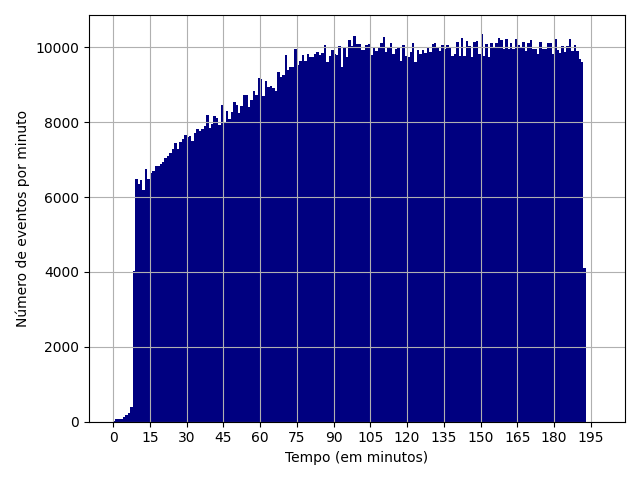
\includegraphics[width=\textwidth]{figuras/graphics/histogram_vazao_9-dez-su.png}
\caption{Vazão de eventos detectados pelo sistema na execução 4 do experimento utilizando o algoritmo de balanceamento por Uso de Estado.}
\label{fig:vazao_9-dez-su}
\end{figure}

%\subsection{Número de instâncias e de eventos de entrada}


\begin{figure}[h]
\centering
\begin{subfigure}{0.9\textwidth}
\centering
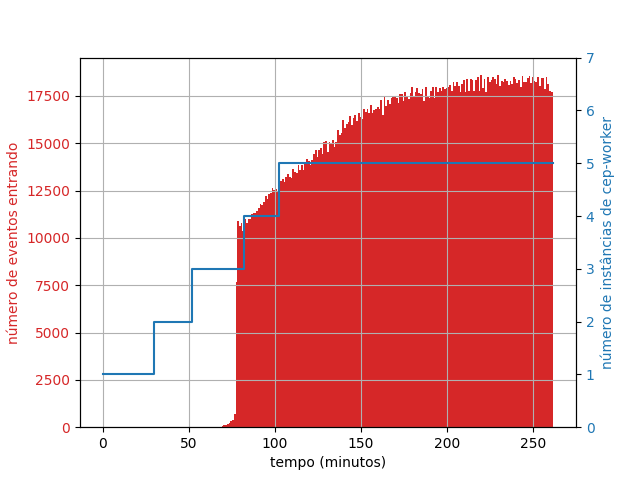
\includegraphics[width=\textwidth]{figuras/graphics/carga_e_workers_total9-dez-su.png}
\caption{Número de eventos entrando no sistema (em vermelho) e número de instâncias de \texttt{CEP Worker} (em azul) em função do tempo na execução 4 do experimento utilizando o algoritmo de balanceamento de carga por Uso de Estado.}
\label{fig:workers_and_load_total_9-dez-su}
\end{subfigure}%

\begin{subfigure}{\textwidth}
\centering
\includegraphics[width=\textwidth]{figuras/graphics/carga_e_workers_horario9-dez-su.png}
\caption{Número de eventos entrando no sistema (em vermelho) e número de instâncias de \texttt{CEP Worker} (em azul) em função do horário do dia na execução 4 do experimento utilizando o algoritmo de balanceamento de carga por Uso de Estado.}
\label{fig:workers_and_load_SPtrans_9-dez-su}
\end{subfigure}%
\caption{Número de eventos entrando no sistema e número de instâncias de \texttt{CEP Worker} na execução 4 do experimento utilizando o algoritmo de balanceamento de carga por Uso de Estado.}
\end{figure}

%\subsection{Latência}


\begin{figure}
\centering
\begin{subfigure}{.5\textwidth}
\centering
\includegraphics[width=\textwidth]{figuras/graphics/boxplot_9-dez-su_vf.png}
\caption{BoxPlot da latência da categoria de tipos de evento \textbf{vf} por intervalos de cinco minutos ao longo da execução 4 do experimento utilizando o algoritmo de balanceamento de carga por Uso de Estado.}
\label{fig:BoxPlot_vf_SU_9-dez-su}
\end{subfigure}%
%\end{figure}

%\begin{figure}
\begin{subfigure}{.5\textwidth}
\centering
\includegraphics[width=\textwidth]{figuras/graphics/boxplot_9-dez-su_vi.png}
\caption{BoxPlot da latência da categoria de tipos de evento \textbf{vi} por intervalos de cinco minutos ao longo da execução 4 do experimento utilizando o algoritmo de balanceamento de carga por Uso de Estado.}
\label{fig:BoxPlot_vi_SU_9-dez-su}
\end{subfigure}%
%\end{figure}
\centering
%\begin{figure}
\begin{subfigure}{.5\textwidth}
\centering
\includegraphics[width=\textwidth]{figuras/graphics/boxplot_9-dez-su_vel.png}
\caption{BoxPlot da latência da categoria de tipos de evento \textbf{vel} por intervalos de cinco minutos ao longo da execução 4 do experimento utilizando o algoritmo de balanceamento de carga por Uso de Estado.}
\label{fig:BoxPlot_vel_SU_9-dez-su}
\end{subfigure}%
%\end{figure}

%\begin{figure}
\begin{subfigure}{.5\textwidth}
\centering
\includegraphics[width=\textwidth]{figuras/graphics/boxplot_9-dez-su_corr.png}
\caption{BoxPlot da latência da categoria de tipos de evento \textbf{corr} por intervalos de cinco minutos ao longo da execução 4 do experimento utilizando o algoritmo de balanceamento de carga por Uso de Estado.}
\label{fig:BoxPlot_corr_SU_9-dez-su}
\end{subfigure}%
%\end{figure}
%\begin{figure}
\begin{subfigure}{.5\textwidth}
\centering
\includegraphics[width=\textwidth]{figuras/graphics/boxplot_9-dez-su_busb.png}
\caption{BoxPlot da latência da categoria de tipos de evento \textbf{BusB} por intervalos de cinco minutos ao longo da execução 4 do experimento utilizando o algoritmo de balanceamento de carga por Uso de Estado.}
\label{fig:BoxPlot_BusB_SU_9-dez-su}
\end{subfigure}%
\caption{BoxPlot da latência por intervalos de cinco minutos ao longo da execução 4 do experimento utilizando o algoritmo de balanceamento de carga por Uso de Estado.}
\end{figure}






%----------------------------------------
%\newpage
%\section{Experimento 4 - Algoritmo de Similaridade de Entrada}

%\subsection{Vazão}


\begin{figure}[h]
\centering
\includegraphics[width=\textwidth]{figuras/graphics/histogram_vazao_9-dez-is.png}
\caption{Vazão de eventos detectados pelo sistema na execução 4 do experimento utilizando o algoritmo de balanceamento por Similaridade de Entrada.}
\label{fig:vazao_9-dez-is}
\end{figure}

%\subsection{Número de instâncias e de eventos de entrada}


\begin{figure}[h]
\centering
\begin{subfigure}{0.9\textwidth}
\centering
\includegraphics[width=\textwidth]{figuras/graphics/carga_e_workers_total9-dez-is.png}
\caption{Número de eventos entrando no sistema (em vermelho) e número de instâncias de \texttt{CEP Worker} (em azul) em função do tempo na execução 4 do experimento utilizando o algoritmo de balanceamento de carga por Similaridade de Entrada.}
\label{fig:workers_and_load_total-9-dez-is}
\end{subfigure}%

\begin{subfigure}{\textwidth}
\centering
\includegraphics[width=\textwidth]{figuras/graphics/carga_e_workers_horario9-dez-is.png}
\caption{Número de eventos entrando no sistema (em vermelho) e número de instâncias de \texttt{CEP Worker} (em azul) em função do horário do dia na execução 4 do experimento utilizando o algoritmo de balanceamento de carga por Similaridade de Entrada.}
\label{fig:workers_and_load_SPtrans-9-dez-is}
\end{subfigure}%
\caption{Número de eventos entrando no sistema e número de instâncias de \texttt{CEP Worker} na execução 5 do experimento utilizando o algoritmo de balanceamento de carga por Similaridade de Entrada.}
\end{figure}






%\subsection{Latência}


\begin{figure}
\centering
\begin{subfigure}{.5\textwidth}
\centering
\includegraphics[width=\textwidth]{figuras/graphics/boxplot_9-dez-is_vf.png}
\caption{BoxPlot da latência da categoria de tipos de evento \textbf{vf} por intervalos de cinco minutos ao longo da execução 4 do experimento utilizando o algoritmo de balanceamento de carga por Similaridade de Entrada.}
\label{fig:BoxPlot_vf_9-dez-is}
\end{subfigure}%
%\end{figure}

%\begin{figure}
\begin{subfigure}{.5\textwidth}
\centering
\includegraphics[width=\textwidth]{figuras/graphics/boxplot_9-dez-is_vi.png}
\caption{BoxPlot da latência da categoria de tipos de evento \textbf{vi} por intervalos de cinco minutos ao longo da execução 4 do experimento utilizando o algoritmo de balanceamento de carga por Similaridade de Entrada.}
\label{fig:BoxPlot_vi_IS_9-dez-is}
\end{subfigure}%
%\end{figure}
\centering
%\begin{figure}
\begin{subfigure}{.5\textwidth}
\centering
\includegraphics[width=\textwidth]{figuras/graphics/boxplot_9-dez-is_vel.png}
\caption{BoxPlot da latência da categoria de tipos de evento \textbf{vel} por intervalos de cinco minutos ao longo da execução 4 do experimento utilizando o algoritmo de balanceamento de carga por Similaridade de Entrada.}
\label{fig:BoxPlot_vel_IS_9-dez-is}
\end{subfigure}%
%\end{figure}

%\begin{figure}
\begin{subfigure}{.5\textwidth}
\centering
\includegraphics[width=\textwidth]{figuras/graphics/boxplot_9-dez-is_corr.png}
\caption{BoxPlot da latência da categoria de tipos de evento \textbf{corr} por intervalos de cinco minutos ao longo da execução 4 do experimento utilizando o algoritmo de balanceamento de carga por Similaridade de Entrada.}
\label{fig:BoxPlot_corr_IS_9-dez-is}
\end{subfigure}%
%\end{figure}
%\begin{figure}
\begin{subfigure}{.5\textwidth}
\centering
\includegraphics[width=\textwidth]{figuras/graphics/boxplot_9-dez-is_busb.png}
\caption{BoxPlot da latência da categoria de tipos de evento \textbf{BusB} por intervalos de cinco minutos ao longo da execução 4 do experimento utilizando o algoritmo de balanceamento de carga por Similaridade de Entrada.}
\label{fig:BoxPlot_BusB_IS_9-dez-is}
\end{subfigure}%
\caption{BoxPlot da latência por intervalos de cinco minutos ao longo da execução 4 do experimento utilizando o algoritmo de balanceamento de carga por Similaridade de Entrada.}
\end{figure}



%--------777777777777777777777777777777777777
%\newpage

%\section{Experimento 5 - Algoritmo de Uso de Estado}

%\subsection{Vazão}


\begin{figure}[h]
\centering
\includegraphics[width=\textwidth]{figuras/graphics/histogram_vazao_10-dez-su.png}
\caption{Vazão de eventos detectados pelo sistema na execução 5 do experimento utilizando o algoritmo de balanceamento por Uso de Estado.}
\label{fig:vazao_9-dez-su}
\end{figure}



%\subsection{Número de instâncias e de eventos de entrada}


\begin{figure}[h]
\centering
\begin{subfigure}{\textwidth}
\centering
\includegraphics[width=0.9\textwidth]{figuras/graphics/carga_e_workers_total10-dez-su.png}
\caption{Número de eventos entrando no sistema (em vermelho) e número de instâncias de \texttt{CEP Worker} (em azul) em função do tempo na execução 5 do experimento utilizando o algoritmo de balanceamento de carga por Uso de Estado.}
\label{fig:workers_and_load_total_10-dez-su}
\end{subfigure}%

\begin{subfigure}{\textwidth}
\centering
\includegraphics[width=\textwidth]{figuras/graphics/carga_e_workers_horario10-dez-su.png}
\caption{Número de eventos entrando no sistema (em vermelho) e número de instâncias de \texttt{CEP Worker} (em azul) em função do horário do dia na execução 5 do experimento utilizando o algoritmo de balanceamento de carga por Uso de Estado.}
\label{fig:workers_and_load_SPtrans_10-dez-su}
\end{subfigure}%
\caption{Número de eventos entrando no sistema e número de instâncias de \texttt{CEP Worker} na execução 5 do experimento utilizando o algoritmo de balanceamento de carga por Uso de Estado.}
\end{figure}



%\subsection{Latência}


\begin{figure}
\centering
\begin{subfigure}{.5\textwidth}
\centering
\includegraphics[width=\textwidth]{figuras/graphics/boxplot_10-dez-su_vf.png}
\caption{BoxPlot da latência da categoria de tipos de evento \textbf{vf} por intervalos de cinco minutos ao longo da execução 5 do experimento utilizando o algoritmo de balanceamento de carga por Uso de Estado.}
\label{fig:BoxPlot_vf_SU_10-dez-su}
\end{subfigure}%
%\end{figure}

%\begin{figure}
\begin{subfigure}{.5\textwidth}
\centering
\includegraphics[width=\textwidth]{figuras/graphics/boxplot_10-dez-su_vi.png}
\caption{BoxPlot da latência da categoria de tipos de evento \textbf{vi} por intervalos de cinco minutos ao longo da execução 5 do experimento utilizando o algoritmo de balanceamento de carga por Uso de Estado.}
\label{fig:BoxPlot_vi_SU_10-dez-su}
\end{subfigure}%
%\end{figure}
\centering
%\begin{figure}
\begin{subfigure}{.5\textwidth}
\centering
\includegraphics[width=\textwidth]{figuras/graphics/boxplot_10-dez-su_vel.png}
\caption{BoxPlot da latência da categoria de tipos de evento \textbf{vel} por intervalos de cinco minutos ao longo da execução 5 do experimento utilizando o algoritmo de balanceamento de carga por Uso de Estado.}
\label{fig:BoxPlot_vel_SU_10-dez-su}
\end{subfigure}%
%\end{figure}

%\begin{figure}
\begin{subfigure}{.5\textwidth}
\centering
\includegraphics[width=\textwidth]{figuras/graphics/boxplot_10-dez-su_corr.png}
\caption{BoxPlot da latência da categoria de tipos de evento \textbf{corr} por intervalos de cinco minutos ao longo da execução 5 do experimento utilizando o algoritmo de balanceamento de carga por Uso de Estado.}
\label{fig:BoxPlot_corr_SU_10-dez-su}
\end{subfigure}%
%\end{figure}
%\begin{figure}
\begin{subfigure}{.5\textwidth}
\centering
\includegraphics[width=\textwidth]{figuras/graphics/boxplot_10-dez-su_busb.png}
\caption{BoxPlot da latência da categoria de tipos de evento \textbf{BusB} por intervalos de cinco minutos ao longo da execução 5 do experimento utilizando o algoritmo de balanceamento de carga por Uso de Estado.}
\label{fig:BoxPlot_BusB_SU_10-dez-su}
\end{subfigure}%
\caption{BoxPlot da latência por intervalos de cinco minutos ao longo da execução 5 do experimento utilizando o algoritmo de balanceamento de carga por Uso de Estado.}
\end{figure}




%----------------------------------------
%\newpage
%\section{Experimento 5 - Algoritmo de Similaridade de Entrada}

%\subsection{Vazão}


\begin{figure}[h]
\centering
\includegraphics[width=\textwidth]{figuras/graphics/histogram_vazao_10-dez-is.png}
\caption{Vazão de eventos detectados pelo sistema na execução 5 do experimento utilizando o algoritmo de balanceamento por Similaridade de Entrada.}
\label{fig:vazao_10-dez-is}
\end{figure}

%\subsection{Número de instâncias e de eventos de entrada}


\begin{figure}[h]
\begin{subfigure}{0.9\textwidth}
\includegraphics[width=\textwidth]{figuras/graphics/carga_e_workers_total10-dez-is.png}
\caption{Número de eventos entrando no sistema (em vermelho) e número de instâncias de \texttt{CEP Worker} (em azul) em função do tempo na execução 5 do experimento utilizando o algoritmo de balanceamento de carga por Similaridade de Entrada.}
\label{fig:workers_and_load_total-10-dez-is}
\end{subfigure}

\begin{subfigure}{\textwidth}
\includegraphics[width=\textwidth]{figuras/graphics/carga_e_workers_horario10-dez-is.png}
\caption{Número de eventos entrando no sistema (em vermelho) e número de instâncias de \texttt{CEP Worker} (em azul) em função do horário do dia na execução 5 do experimento utilizando o algoritmo de balanceamento de carga por Similaridade de Entrada.}
\label{fig:workers_and_load_SPtrans-10-dez-is}
\end{subfigure}%
\end{figure}



%\subsection{Latência}


\begin{figure}
\centering
\begin{subfigure}{.5\textwidth}
\centering
\includegraphics[width=\textwidth]{figuras/graphics/boxplot_10-dez-is_vf.png}
\caption{BoxPlot da latência da categoria de tipos de evento \textbf{vf} por intervalos de cinco minutos ao longo da execução 5 do experimento utilizando o algoritmo de balanceamento de carga por Similaridade de Entrada.}
\label{fig:BoxPlot_vf_10-dez-is}
\end{subfigure}%
%\end{figure}

%\begin{figure}
\begin{subfigure}{.5\textwidth}
\centering
\includegraphics[width=\textwidth]{figuras/graphics/boxplot_10-dez-is_vi.png}
\caption{BoxPlot da latência da categoria de tipos de evento \textbf{vi} por intervalos de cinco minutos ao longo da execução 5 do experimento utilizando o algoritmo de balanceamento de carga por Similaridade de Entrada.}
\label{fig:BoxPlot_vi_IS_10-dez-is}
\end{subfigure}%
%\end{figure}
\centering
%\begin{figure}
\begin{subfigure}{.5\textwidth}
\centering
\includegraphics[width=\textwidth]{figuras/graphics/boxplot_10-dez-is_vel.png}
\caption{BoxPlot da latência da categoria de tipos de evento \textbf{vel} por intervalos de cinco minutos ao longo da execução 5 do experimento utilizando o algoritmo de balanceamento de carga por Similaridade de Entrada.}
\label{fig:BoxPlot_vel_IS_10-dez-is}
\end{subfigure}%
%\end{figure}

%\begin{figure}
\begin{subfigure}{.5\textwidth}
\centering
\includegraphics[width=\textwidth]{figuras/graphics/boxplot_10-dez-is_corr.png}
\caption{BoxPlot da latência da categoria de tipos de evento \textbf{corr} por intervalos de cinco minutos ao longo da execução 5 do experimento utilizando o algoritmo de balanceamento de carga por Similaridade de Entrada.}
\label{fig:BoxPlot_corr_IS_10-dez-is}
\end{subfigure}%
%\end{figure}
%\begin{figure}
\begin{subfigure}{.5\textwidth}
\centering
\includegraphics[width=\textwidth]{figuras/graphics/boxplot_10-dez-is_busb.png}
\caption{BoxPlot da latência da categoria de tipos de evento \textbf{BusB} por intervalos de cinco minutos ao longo da execução 5 do experimento utilizando o algoritmo de balanceamento de carga por Similaridade de Entrada.}
\label{fig:BoxPlot_BusB_IS_10-dez-is}
\end{subfigure}%
\caption{BoxPlot da latência por intervalos de cinco minutos ao longo da execução 5 do experimento utilizando o algoritmo de balanceamento de carga por Similaridade de Entrada.}
\end{figure}




%\section{Velocidade média ao longo do horário nos corredores de ônibus}
\newpage

%\section{Velocidade média de cada corredor pelo horário da SPTrans}

\begin{figure}[ht]
\centering
\begin{subfigure}{.45\textwidth}
  \centering
  \includegraphics[width=\textwidth]{figuras/detect_graphics/avg_speed_7-dez-su-corr_Ibirapuera.png}
  \caption{Ibirapuera.}
  \label{fig::avg_speed_Ibirapuera}
\end{subfigure}%
\begin{subfigure}{.45\textwidth}
  \centering
  \includegraphics[width=\textwidth]{figuras/detect_graphics/avg_speed_7-dez-su-corr_Inajar.png}
  \caption{Inajar.}
  \label{fig::avg_speed_Inajar}
\end{subfigure}
%\end{figure}
%\begin{figure}
\centering
\begin{subfigure}{.45\textwidth}
  \centering
  \includegraphics[width=\textwidth]{figuras/detect_graphics/avg_speed_7-dez-su-corr_Pirituba.png}
  \caption{Pirituba.}
  \label{fig::avg_speed_Pirituba}
\end{subfigure}%
\begin{subfigure}{.45\textwidth}
  \centering
  \includegraphics[width=\textwidth]{figuras/detect_graphics/avg_speed_7-dez-su-corr_PonteBaixa.png}
  \caption{Ponte Baixa.}
  \label{fig::avg_speed_Ponte_Baixa}
\end{subfigure}
%\end{figure}
%\begin{figure}
\centering
\begin{subfigure}{.45\textwidth}
  \centering
\includegraphics[width=\textwidth]{figuras/detect_graphics/avg_speed_7-dez-su-corr_Itapecerica.png}
\caption{Itapecirica.}
\label{fig::avg_speed_Itapecirica}
\end{subfigure}%
\begin{subfigure}{.45\textwidth}
 \centering
 \includegraphics[width=\textwidth]{figuras/detect_graphics/avg_speed_7-dez-su-corr_NoveDeJulho.png}
 \caption{Nove De Julho.}
 \label{fig::avg_speed_Nove_de_Julho}
\end{subfigure}
 \caption{Velocidade média de cada corredor detectada pelos tipos de eventos da categoria \textbf{corr} ao longo do horário do dia de coleta dos dados.}
\end{figure}
\begin{figure}
\centering
\begin{subfigure}{.5\textwidth}
  \centering
\includegraphics[width=\textwidth]{figuras/detect_graphics/avg_speed_7-dez-su-corr_Tiradentes.png}
\caption{Tiradentes.}
\label{fig::avg_speed_Tiradentes}
\end{subfigure}%
\begin{subfigure}{.5\textwidth}
 \centering
 \includegraphics[width=\textwidth]{figuras/detect_graphics/avg_speed_7-dez-su-corr_Guarapiranga.png}
 \caption{Guarapiranga.}
 \label{fig::avg_speed_Guarapiranga}
\end{subfigure}
%\end{figure}
%\begin{figure}[ht]
\centering
\begin{subfigure}{.5\textwidth}
  \centering
  \includegraphics[width=\textwidth]{figuras/detect_graphics/avg_speed_7-dez-su-corr_Berrini.png}
  \caption{Berrini.}
  \label{fig:avg_speed_Berrini}
\end{subfigure}%
\begin{subfigure}{.5\textwidth}
  \centering
  \includegraphics[width=\textwidth]{figuras/detect_graphics/avg_speed_7-dez-su-corr_CampoLimpo.png}
  \caption{Campo Limpo.}
  \label{fig:avg_speed_Campo Limpo}
\end{subfigure}
%\end{figure}
%\begin{figure}
\centering
\begin{subfigure}{.5\textwidth}
  \centering
  \includegraphics[width=\textwidth]{figuras/detect_graphics/avg_speed_7-dez-su-corr_PaesDeBarros.png}
  \caption{Paes de Barros.}
  \label{fig::avg_speed_Paes_de_Barros}
\end{subfigure}%
\begin{subfigure}{.5\textwidth}
  \centering
  \includegraphics[width=\textwidth]{figuras/detect_graphics/avg_speed_7-dez-su-corr_Parelheiros.png}
  \caption{Parelheiros.}
  \label{fig::avg_speed_Parelheiros}
\end{subfigure}
 \caption{Velocidade média de cada corredor detectada pelos tipos de eventos da categoria \textbf{corr} ao longo do horário do dia de coleta dos dados.}
\label{fig:all_avg_speed_corr}
\end{figure}





\begin{comment}
\begin{figure}[ht]
\centering
\begin{subfigure}{.5\textwidth}
  \centering
  \includegraphics[width=\textwidth]{figuras/graphics/boxplot_5-dez-su_vf.png}
  \caption{repetição 1 - Uso de Estado}
  \label{fig:BoxPlot_vf_SU_1}
\end{subfigure}%
\begin{subfigure}{.5\textwidth}
  \centering
  \includegraphics[width=\textwidth]{figuras/graphics/boxplot_6-dez-is_vf.png}
  \caption{repetição 1 - Similaridade de Entrada}
  \label{fig:BoxPlot_vf_IS_1}
\end{subfigure}
%\end{figure}
%\begin{figure}
\centering
\begin{subfigure}{.5\textwidth}
  \centering
  \includegraphics[width=\textwidth]{figuras/graphics/boxplot_5-dez-su_vf.png}
  \caption{repetição 1 - Uso de Estado}
  \label{fig:BoxPlot_vf_SU_2}
\end{subfigure}%
\begin{subfigure}{.5\textwidth}
  \centering
  \includegraphics[width=\textwidth]{figuras/graphics/boxplot_6-dez-is_vf.png}
  \caption{repetição 1 - Similaridade de Entrada}
  \label{fig:BoxPlot_vf_IS_2}
\end{subfigure}
\end{figure}

\begin{figure}[ht]
\centering
\begin{subfigure}{.5\textwidth}
  \centering
  \includegraphics[width=\textwidth]{figuras/graphics/boxplot_5-dez-su_vf.png}
  \caption{repetição 1 - Uso de Estado}
  \label{fig:BoxPlot_vf_SU_3}
\end{subfigure}%
\begin{subfigure}{.5\textwidth}
  \centering
  \includegraphics[width=\textwidth]{figuras/graphics/boxplot_6-dez-is_vf.png}
  \caption{repetição 1 - Similaridade de Entrada}
  \label{fig:BoxPlot_vf_IS_3}
\end{subfigure}
%\end{figure}
%\begin{figure}
\centering
\begin{subfigure}{.5\textwidth}
  \centering
\includegraphics[width=\textwidth]{figuras/graphics/boxplot_8-dez-su_vf.png}
\caption{repetição 3 - Uso de Estado}
\label{fig:BoxPlot_vf_SU_4}
\end{subfigure}%
\begin{subfigure}{.5\textwidth}
 \centering
 \includegraphics[width=\textwidth]{figuras/graphics/boxplot_8-dez-is_vf.png}
 \caption{repetição 3 - Similaridade de Entrada}
 \label{fig:BoxPlot_vf_IS_4}
\end{subfigure}
%\end{figure}
%\begin{figure}
\centering
\begin{subfigure}{.5\textwidth}
  \centering
\includegraphics[width=\textwidth]{figuras/graphics/boxplot_8-dez-su_vf.png}
\caption{repetição 4 - Uso de Estado}
\label{fig:BoxPlot_vf_SU_5}
\end{subfigure}%
\begin{subfigure}{.5\textwidth}
 \centering
 \includegraphics[width=\textwidth]{figuras/graphics/boxplot_8-dez-is_vf.png}
 \caption{repetição 4 - Similaridade de Entrada}
 \label{fig:BoxPlot_vf_IS_5}
\end{subfigure}
\end{figure}




\section{Latência mediana dos eventos de filtro de velocidade}

\begin{figure}[]ht
\centering
\begin{subfigure}{.5\textwidth}
  \centering
\includegraphics[width=\textwidth]{figuras/graphics/carga_e_workers_horario7-dez-su.png}
\caption{Número de Workers por horário da carga}
\label{fig:BoxPlot_busb+20_1}
\end{subfigure}%
\begin{subfigure}{.5\textwidth}
 \centering
 \includegraphics[width=\textwidth]{figuras/graphics/carga_e_workers_total7-dez-su.png}
 \caption{Número de Workers por tempo total}
 \label{fig:BoxPlot_busb-20_1}
\end{subfigure}
\end{figure}

\section{Latência mediana dos eventos de velocidade média dos ônibus que passam em corredores}



\section{Latência mediana dos eventos de velocidade média dos corredores de ônibus}




\section{Latência mediana dos eventos de Agrupamento de ônibus}



\section{Número de Instâncias de CEP Worker e carga de eventos de entrada pelo tempo}


\section{Número de Instâncias de CEP Worker e carga de eventos de entrada pelo horário da SPTrans}




%\begin{comment}
\singlespacing

\renewcommand{\arraystretch}{0.85}
\captionsetup{margin=1.0cm}  % correção nas margens dos captions.
%--------------------------------------------------------------------------------------
\begin{table}
\begin{center}
\begin{small}
\begin{tabular}{|c|c|c|c|c|c|c|c|c|c|c|c|c|} 
\hline
\emph{Limiar} & 
\multicolumn{3}{c|}{MGWT} & 
\multicolumn{3}{c|}{AMI} &  
\multicolumn{3}{c|}{\emph{Spectrum} de Fourier} & 
\multicolumn{3}{c|}{Características espectrais} \\
\cline{2-4} \cline{5-7} \cline{8-10} \cline{11-13} & 
\emph{Sn} & \emph{Sp} & \emph{AC} & 
\emph{Sn} & \emph{Sp} & \emph{AC} & 
\emph{Sn} & \emph{Sp} & \emph{AC} & 
\emph{Sn} & \emph{Sp} & \emph{AC}\\ \hline \hline
 1 & 1.00 & 0.16 & 0.08 & 1.00 & 0.16 & 0.08 & 1.00 & 0.16 & 0.08 & 1.00 & 0.16 & 0.08 \\
 2 & 1.00 & 0.16 & 0.09 & 1.00 & 0.16 & 0.09 & 1.00 & 0.16 & 0.09 & 1.00 & 0.16 & 0.09 \\
 2 & 1.00 & 0.16 & 0.10 & 1.00 & 0.16 & 0.10 & 1.00 & 0.16 & 0.10 & 1.00 & 0.16 & 0.10 \\
 4 & 1.00 & 0.16 & 0.10 & 1.00 & 0.16 & 0.10 & 1.00 & 0.16 & 0.10 & 1.00 & 0.16 & 0.10 \\
 5 & 1.00 & 0.16 & 0.11 & 1.00 & 0.16 & 0.11 & 1.00 & 0.16 & 0.11 & 1.00 & 0.16 & 0.11 \\
 6 & 1.00 & 0.16 & 0.12 & 1.00 & 0.16 & 0.12 & 1.00 & 0.16 & 0.12 & 1.00 & 0.16 & 0.12 \\
 7 & 1.00 & 0.17 & 0.12 & 1.00 & 0.17 & 0.12 & 1.00 & 0.17 & 0.12 & 1.00 & 0.17 & 0.13 \\
 8 & 1.00 & 0.17 & 0.13 & 1.00 & 0.17 & 0.13 & 1.00 & 0.17 & 0.13 & 1.00 & 0.17 & 0.13 \\
 9 & 1.00 & 0.17 & 0.14 & 1.00 & 0.17 & 0.14 & 1.00 & 0.17 & 0.14 & 1.00 & 0.17 & 0.14 \\
10 & 1.00 & 0.17 & 0.15 & 1.00 & 0.17 & 0.15 & 1.00 & 0.17 & 0.15 & 1.00 & 0.17 & 0.15 \\
11 & 1.00 & 0.17 & 0.15 & 1.00 & 0.17 & 0.15 & 1.00 & 0.17 & 0.15 & 1.00 & 0.17 & 0.15 \\
12 & 1.00 & 0.18 & 0.16 & 1.00 & 0.18 & 0.16 & 1.00 & 0.18 & 0.16 & 1.00 & 0.18 & 0.16 \\
13 & 1.00 & 0.18 & 0.17 & 1.00 & 0.18 & 0.17 & 1.00 & 0.18 & 0.17 & 1.00 & 0.18 & 0.17 \\
14 & 1.00 & 0.18 & 0.17 & 1.00 & 0.18 & 0.17 & 1.00 & 0.18 & 0.17 & 1.00 & 0.18 & 0.17 \\
15 & 1.00 & 0.18 & 0.18 & 1.00 & 0.18 & 0.18 & 1.00 & 0.18 & 0.18 & 1.00 & 0.18 & 0.18 \\
16 & 1.00 & 0.18 & 0.19 & 1.00 & 0.18 & 0.19 & 1.00 & 0.18 & 0.19 & 1.00 & 0.18 & 0.19 \\
17 & 1.00 & 0.19 & 0.19 & 1.00 & 0.19 & 0.19 & 1.00 & 0.19 & 0.19 & 1.00 & 0.19 & 0.19 \\
17 & 1.00 & 0.19 & 0.20 & 1.00 & 0.19 & 0.20 & 1.00 & 0.19 & 0.20 & 1.00 & 0.19 & 0.20 \\
19 & 1.00 & 0.19 & 0.21 & 1.00 & 0.19 & 0.21 & 1.00 & 0.19 & 0.21 & 1.00 & 0.19 & 0.21 \\
20 & 1.00 & 0.19 & 0.22 & 1.00 & 0.19 & 0.22 & 1.00 & 0.19 & 0.22 & 1.00 & 0.19 & 0.22 \\ \hline 
\end{tabular}
\caption{Exemplo de tabela.}
\label{tab:tab:F5}
\end{small}
\end{center}
\end{table}

\end{comment}      



% associado ao arquivo: 'ape-conjuntos.tex'

% ---------------------------------------------------------------------------- %
% Bibliografia
\backmatter \singlespacing   % espaçamento simples
\bibliographystyle{plainnat-ime} % citação bibliográfica textual
\bibliography{bibliografia}  % associado ao arquivo: 'bibliografia.bib'

% ---------------------------------------------------------------------------- %
% Índice remissivo
%\index{TBP|see{periodicidade região codificante}}
%\index{DSP|see{processamento digital de sinais}}
%\index{STFT|see{transformada de Fourier de tempo reduzido}}
%\index{DFT|see{transformada discreta de Fourier}}
%\index{Fourier!transformada|see{transformada de Fourier}}

\printindex   % imprime o índice remissivo no documento 

\end{document}
